\documentclass[logos,hyperref,mainlanguage=english,morelanguage=french]{my-orsay-thesis}
%Text encoding and fonts
\usepackage[latin1]{inputenc}
\usepackage[T1]{fontenc}
\usepackage{amsmath}
\usepackage{mathrsfs}
\usepackage{cancel}
\usepackage{caption}
\usepackage{subcaption}
% \bibliographystyle{unsrt}
\usepackage[hyperref=true,
            url=false,
            isbn=false,
            backref=true,
            maxcitenames=3,
            maxbibnames=100,
            block=none,
            style=trad-unsrt,
            backend=biber]{biblatex}
\bibliography{./bib/biblio}
\DefineBibliographyStrings{english}{%
    backrefpage  = {see p.}, % for single page number
    backrefpages = {see pp.} % for multiple page numbers
}
\usepackage[activate={true,nocompatibility},final,tracking=true,kerning=true,spacing=true,factor=1100,stretch=10,shrink=10]{microtype}
% activate={true,nocompatibility} - activate protrusion and expansion
% final - enable microtype; use "draft" to disable
% tracking=true, kerning=true, spacing=true - activate these techniques
% factor=1100 - add 10% to the protrusion amount (default is 1000)
% stretch=10, shrink=10 - reduce stretchability/shrinkability (default is 20/20)
\SetTracking{encoding={*}, shape=sc}{40}
\SetProtrusion{encoding={*},family={bch},series={*},size={6,7}}
              {1={ ,750},2={ ,500},3={ ,500},4={ ,500},5={ ,500},
               6={ ,500},7={ ,600},8={ ,500},9={ ,500},0={ ,500}}
\graphicspath{{./figures/}}
%########################################################################
% Title page
%########################################################################
\author{Oscar Roberto \textsc{BLANCO GARC�A}}
\title{Beam dynamics in the final focus of the CLIC future linear collider project}
\title[english]{Dynamique du faisceau dans las section finale de focalisation du futur collissionneur lin�aire}
\keywords{Some keywords}
%Keywords for other languages languages
% \keywords[english]{Blabla, blabla, blabla, blabla, blabla, blabla, blabla}
%Order number of the thesis
\ordernumber{xxxx}
%Date of defense
\date{3 juillet 2015}
%You define the commission member list using \addcommissionmember (mandatory) with an optional role (eg: president, supervisor, etc...)
\addcommissionmember[Directeur de th�se]{M.}{Philip}{Bambade}
\addcommissionmember[Codirecteur de th�se]{M.}{Rogelio}{Tom�s}
\addcommissionmember{M.}{Toshiaki}{Tauchi}
\addcommissionmember[Pr�sident du jury]{M.}{Iiii}{Jjjjjjjjjjjj}
%If some referees are not part of the commission, you can add them in a separate list with \addreferee (optional)
\addreferee{M.}{Jean-Marie}{DE CONTO}
\addreferee{M.}{Nobuhiro}{TERUNUMA}
%########################################################################
% Document start
%########################################################################
\begin{document}
%Print title NOW
\maketitle%
%Disable page numbering
\pagestyle{empty}
%########################################################################
% Multilingual abstracts
%########################################################################
% %French abstract:
% \begin{abstract}
% \begin{abstract}[english]
The exploration of new physics in the TeV scale with precision measurements requires lepton colliders providing high luminosities to obtain enough statistics for the data analysis. In order to achieve design luminosity values, linear colliders feature nanometer beam spot sizes at the Interaction~Point~(IP).\par
In addition to several effects affecting the luminosity, three main issues to achieve the beam size demagnification in the Final Focus Section (FFS) of the accelerator are the chromaticity correction, the synchrotron radiation effects and the correction of the lattice errors.\par
The current linear collider projects, CLIC and ILC, have lattices designed using the local or non-local chromaticity correction schemes. A new chromaticity correction scheme, called non-interleaved, is proposed to the local and non-local chromaticity corrections for CLIC. This lattice is designed and diagnosed, where the main issue in the current state of lattice design is the non-zero second order dispersion in the Final Doublet~(FD) region where a strong sextupole is used to correct the remaining geometrical components. It could be solved by cancelling the second order dispersion and its derivative before the FD.\par
The radiation effect can be evaluated by tracking particles through the lattice or by analytical approximations during the design stage of the lattices. In order to include both, radiation and optic parameters, during the design optimization process, two particular radiation phenomena are reviewed: the Oide effect~\cite{Oide} and the radiation caused by bending magnets~\cite{Sands}.\par
The analytical result of the radiation in bending magnets in~\cite{Sands} was generalized to the case with non-zero alpha and non-zero dispersion at the IP, required during the design and luminosity optimization process. The closed solution for one dipole and one dipole with a drift is compared with the tracking code PLACET~\cite{Placet}, resulting in the improvement of the tracking code results.\par% Finally the model validity for the FFS design is analyzed concluding an agreement within $\pm10\%$ between the theoretical contribution to beam size and the tracking.\par
In the Oide effect, radiation in the final quadrupole sets a limit on the vertical beamsize. Only for CLIC 3~TeV this limit is significant, therefore two possibilities are explored to mitigate its contribution to beam size: double the length and reduce the QD0 gradient, or the integration of a pair of octupoles before and after QD0.\par
% The best result with octupoles demonstrates vertical beam size reduction of $(4.3\pm0.5)$\%, with little or negative impact on luminosity. The correction scheme is currently limited by the phase advance and $\beta_y/\beta_x$ ratio between correctors. It may be possible to improve its performance by slicing QD0.\par
Part of the requirements of the FFS for new linear accelerators, in particular ILC, are tested in The Accelerator Test Facility (ATF). The beam size reduction using the local chromaticity correction is explored by an extension of the original design, called ATF2 with two goals: ({\textbf{goal 1}}) achieve 37~nm of vertical beam size at the IP and ({\textbf{goal 2}}) the stabilization of the IP beam position at the level of few nanometres. Since 2014 beam size of 44~nm are achieved as a regular basis at charges of about~$0.1\times10^{10}$ particules per bunch.\par
A set of three cavities (IPA, IPB and IPC), two upstream and one downstream of the nominal IP, were installed and are used to measure the beam trajectory in the IP region, thus providing enough information to reconstruct the bunch position and angle at the IP. These will be used to for beam stabilization and could detect beam drift/jitter beyond the tolerable margin and undetected optics mismatch affecting the beam size measurements.\par
The specifications required of 1~nm resolution over 10~$\mu$m dynamic range at $1.0\times10^{10}$ particules per bunch with the ATF2 nominal optics have not been yet achieved. The results of the studies in the vertical plane of the cavities calibration show linearity within 5\% over two orders of magnitude of signal attenuation. The minimum resolution achieved is just below 50~nm at~$0.4\times10^{10}$ particules per bunch with a set of electronics impossing a noise limit on resolution of 10~nm per cavity. The dynamic range is 10~$\mu$m at 10~dB attenuation and $0.4\times10^{10}$ particules per bunch, indicating the need to upgrade the electronics. The integration to the ATF tuning instruments is ongoing. Nonetheless, feedback has been tested resulting in reduction of beam jitter down to 67~nm, compatible with resolution.\par
Two improvements have been done on the system since this study. First, the horizontal and vertical planes can be analyzed simultaneouly, such that data can be checked for coupling from one plane to another. Second, filters are added to the system in order to reduce the effect of the mismatch between frequencies in the electronics down-mixing process.\par
\end{abstract}
% \end{abstract}
%Horizontal rule
\noindent\hspace*{0.35\textwidth}\hrulefill\hspace*{0.35\textwidth}\\[-\bigskipamount]
%English abstract:
\begin{abstract}[english]
\begin{abstract}[english]
The exploration of new physics in the TeV scale with precision measurements requires lepton colliders providing high luminosities to obtain enough statistics for the data analysis. In order to achieve design luminosity values, linear colliders feature nanometer beam spot sizes at the Interaction~Point~(IP).\par
In addition to several effects affecting the luminosity, three main issues to achieve the beam size demagnification in the Final Focus Section (FFS) of the accelerator are the chromaticity correction, the synchrotron radiation effects and the correction of the lattice errors.\par
The current linear collider projects, CLIC and ILC, have lattices designed using the local or non-local chromaticity correction schemes. A new chromaticity correction scheme, called non-interleaved, is proposed to the local and non-local chromaticity corrections for CLIC. This lattice is designed and diagnosed, where the main issue in the current state of lattice design is the non-zero second order dispersion in the Final Doublet~(FD) region where a strong sextupole is used to correct the remaining geometrical components. It could be solved by cancelling the second order dispersion and its derivative before the FD.\par
The radiation effect can be evaluated by tracking particles through the lattice or by analytical approximations during the design stage of the lattices. In order to include both, radiation and optic parameters, during the design optimization process, two particular radiation phenomena are reviewed: the Oide effect~\cite{Oide} and the radiation caused by bending magnets~\cite{Sands}.\par
The analytical result of the radiation in bending magnets in~\cite{Sands} was generalized to the case with non-zero alpha and non-zero dispersion at the IP, required during the design and luminosity optimization process. The closed solution for one dipole and one dipole with a drift is compared with the tracking code PLACET~\cite{Placet}, resulting in the improvement of the tracking code results.\par% Finally the model validity for the FFS design is analyzed concluding an agreement within $\pm10\%$ between the theoretical contribution to beam size and the tracking.\par
In the Oide effect, radiation in the final quadrupole sets a limit on the vertical beamsize. Only for CLIC 3~TeV this limit is significant, therefore two possibilities are explored to mitigate its contribution to beam size: double the length and reduce the QD0 gradient, or the integration of a pair of octupoles before and after QD0.\par
% The best result with octupoles demonstrates vertical beam size reduction of $(4.3\pm0.5)$\%, with little or negative impact on luminosity. The correction scheme is currently limited by the phase advance and $\beta_y/\beta_x$ ratio between correctors. It may be possible to improve its performance by slicing QD0.\par
Part of the requirements of the FFS for new linear accelerators, in particular ILC, are tested in The Accelerator Test Facility (ATF). The beam size reduction using the local chromaticity correction is explored by an extension of the original design, called ATF2 with two goals: ({\textbf{goal 1}}) achieve 37~nm of vertical beam size at the IP and ({\textbf{goal 2}}) the stabilization of the IP beam position at the level of few nanometres. Since 2014 beam size of 44~nm are achieved as a regular basis at charges of about~$0.1\times10^{10}$ particules per bunch.\par
A set of three cavities (IPA, IPB and IPC), two upstream and one downstream of the nominal IP, were installed and are used to measure the beam trajectory in the IP region, thus providing enough information to reconstruct the bunch position and angle at the IP. These will be used to for beam stabilization and could detect beam drift/jitter beyond the tolerable margin and undetected optics mismatch affecting the beam size measurements.\par
The specifications required of 1~nm resolution over 10~$\mu$m dynamic range at $1.0\times10^{10}$ particules per bunch with the ATF2 nominal optics have not been yet achieved. The results of the studies in the vertical plane of the cavities calibration show linearity within 5\% over two orders of magnitude of signal attenuation. The minimum resolution achieved is just below 50~nm at~$0.4\times10^{10}$ particules per bunch with a set of electronics impossing a noise limit on resolution of 10~nm per cavity. The dynamic range is 10~$\mu$m at 10~dB attenuation and $0.4\times10^{10}$ particules per bunch, indicating the need to upgrade the electronics. The integration to the ATF tuning instruments is ongoing. Nonetheless, feedback has been tested resulting in reduction of beam jitter down to 67~nm, compatible with resolution.\par
Two improvements have been done on the system since this study. First, the horizontal and vertical planes can be analyzed simultaneouly, such that data can be checked for coupling from one plane to another. Second, filters are added to the system in order to reduce the effect of the mismatch between frequencies in the electronics down-mixing process.\par
\end{abstract}
\end{abstract}
\pagebreak
% %German abstract:
% \begin{abstract}[german]
% \dummytext
% \end{abstract}
%Horizontal rule
\noindent\hspace*{0.35\textwidth}\hrulefill\hspace*{0.35\textwidth}\\[-\bigskipamount]
%########################################################################
% Acknowledgments
%########################################################################
\pagebreak\strut\newpage
\section*{Remerciements}
%Put the text vertically centered
\vfill
This is the night of the 10th of april 2015.\par
I'm at Gen\`eve and I've been just been kicked out from La Petite Reine because the place was closing :'D, as if I care. After two beers here are my deepest acknowledgements:
From the begining...\par
My acknowledgement to Davide, the only person who has been cool every time I talk to him. My deepest acknowledgements to Alex, I wonder how the ILC course would be if I hadn't a person to talk about how people in relationships are like airplains ... some take off in very small tarmacs, like helicopters, some others need a large starting to take off.\par
My acknowledgements to Nuria who is the most constant person in my life during the last 3 years. I hope she has got something good for her life from my way of living. My acknowledgements to Julia, the russian ... waaaaw, life feels hot and nice when you speak to her. My acknowledgement to Hector, that guy is going to have his signature in the world when CLIC-like lattices were built, I want to say that we admire Carl Sagan equally... I thought it would never happen. I want to acknowledge Javier, he is the person who get me into accelerators and it is the only subject I've been looking forward to do things for during the last 10 years. I want to send an special acknowledge to Marcin, the thrill of changing every day for our own sake is what moves us, I would like to have his energy to do stuff, cheers my friend. And now, Tenar the spanish girl who appeared in the moment I most enjoyed it. Tenar, my life and heart is always happy when I hear from you. My biggest love during all these years, Claire. I don't know why, but that is probably the reason why my heart keeps beating when no one is around.\par
I want to thank Rogelio my director in CERN, the dynamics of his day to day is so dedicated to inspire people. Now, Philip, my director at LAL who is the person who stands for all what is right... I always admire how clear the world is for him. Of course, Andrea and Daniel, you are also here ! Daniel, the guy who knows everything about everything, so mind blowing. And Andrea, with whom would I talk about rare films and work at the same time... of course, only Andrea.\par
Finally, to all readers. Precisely today I wanted to be with Claire in the sunny afternoon, and this document kept me away from doing so. It is the moment to get right to the point, clear and neat. I know that Claire is fine, she always is... damn I love that girl.\par
All this is because of you, the reader.\par
N.B. Of course there has been some up and downs, but who cares. Time to flight !
\vfill
\newpage
%########################################################################
% Contents
%########################################################################
\strut\newpage
\microtypesetup{protrusion=false}
\tableofcontents
\listoffigures
\listoftables
\microtypesetup{protrusion=true}
\newpage
%########################################################################
% Introduction
%########################################################################
%Enable page numbering
\pagestyle{fancy}
\chapter*{Introduction}
\addcontentsline{toc}{chapter}{Introduction}
\chapter*{Introduction}
\addcontentsline{toc}{chapter}{Introduction}
The triumph of the 20th century particle physics was the development of the Standard Model. Experiments determined the particle constituents of ordinary matter, and identified four forces binding matter and transforming it from one form to another. This success leads particle physicist to address even more fundamental questions, and explore deeper mysteries in science.\par
The Standard Model includes a third component beyond particles and forces, the Higgs mechanism. The Higgs mechanism permeates the universe, giving mass to the particles, and breaking the electro-weak force in two, the electromagnetic and the weak forces.\par
\begin{figure}[!hbt]
\centering
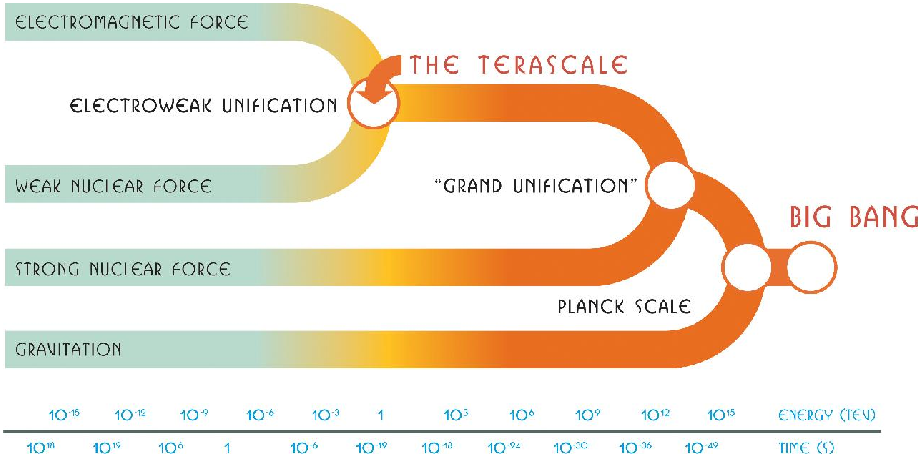
\includegraphics[scale=0.8,angle=0]{energyforce.pdf}\caption{The electromagnetic and electro-weak forces unify at the Terascale.}\label{f:energyforce}
\end{figure}
Experiments in the Terascale could test the idea that fundamental forces originate from a single unified force, see Fig. \ref{f:energyforce}, and search for evidence of a related unified origin of matter involving supersymmetry. They could distinguish among patterns of phenomena to judge different unification models, providing a telescopic view of the ultimate unification.\par
% \section*{The exploration of high energy physics}
% \addcontentsline{toc}{section}{The exploration of high energy physics}
There are two ways to explore the subatomic world, the first is to go to higher energy to discover new particles and measure their properties, the second is to increase the precision of the measurements to detect rare processes and make detailed studies.\par
The LHC allows the exploration of the electroweak symmetry breaking mechanism and other physical phenomena at the TeV scale, like the CP violation problem, the quark gluon plasma at the search of new physics beyond the Standard Model such as supersymmetry (SUSY) among others. The future linear collider beam energy will be determined by the LHC discoveries.\par
\textbf{Higgs searches:} The 4th of July of 2012, in a seminar held at CERN, the collaborations of the Experiments CMS and ATLAS presented an update of the Higgs of the Higgs searches status. At a confidence level of 4.9$\sigma$ for CMS \cite{TheCMSCollaboration21122012}, and 5.1$\sigma$ for ATLAS \cite{TheATLASCollaboration21122012} from the Higgsless Standard Model, signals of a boson with a mass around $m_h=125$~GeV were found with a strong spin-0 indication and coupling parameters consistent with the properties of the Standard Model Higgs Particle. First results on various rare production decay modes have been obtained but more data is needed to observe these models. Many analyses are ongoing and more updates are constantly presented.\par
\textbf{Heavy Flavour and CP Violation:} The experiments of the LHC, led by the LHCb, have carried out several important findings and measurements in the heavy flavour sector. New previously unobserved states have been observed for the very first time during the last years like the states $X_b$, $\Xi_a$ and $\Lambda_s^0$. Also the measurement of the quantum numbers of the states $X(3872)$ with $J^{PC}=1^{++}$, have been determined to the 8$\sigma$ level. The CP violation of the oscillation in D and B mesons have been measured to the 9.1$\sigma$ confidence level discovering the same violation in $B_s$ systems. The CP angle $\gamma$ is known with a precision without precedents ($\gamma=(67\pm12)$\textdegree). Finally, some very rare decays like $B_s\rightarrow\mu^+\mu^-$, $B^0\rightarrow K^*\mu^+\mu^-$ and $D_s^+\rightarrow\pi^+\mu^+\mu^-$ have been observed, with possible implications on the analysis of new physics.\par
\textbf{Quark-gluon Plasma:} The quark-gluon plasma is produced in ultra-relativistic heavy ion collisions. The conditions observed at the LHC experiments (ALICE, ATLAS and CMS) are in agreement with the observations carried out at RHIC. It has been confirmed that the hydrodynamics model helps in the understanding of the behaviour of the processes occurred during the collision. It is still far from being completely understood.\par
\textbf{SUSY and Dark Matter searches:} One of the problem that arises is the stabilization of the Higgs mass and its divergence when quantum divergence is considered. The solution involves a new principle of nature called supersymmetry (SUSY), a new symmetry that unifies bosons and fermions. After data collected during 2011 and 2012, SUSY searches at the LHC did not find any evidence of any light superpartner (squark or gluino) and it has pushed their mass limits beyond 1~TeV with the constrained model~\cite{Kraml:2012er}.\par
\vspace*{0.6cm}
The Second run of the LHC at 13~TeV will provide more information about the physics at high energies.\par

\section*{Circular or linear colliders}
\addcontentsline{toc}{section}{Circular or linear colliders}
Higher energies have been usually explored with hadron colliders and the precision measurements has been done afterwards by lepton colliders, however, lepton circular colliders are limited by radiation. When particles traverse magnetic fields they emmit photons and this photons make the beam loose energy per turn given by
\begin{equation}
 \Delta E_{turn}=\frac{E^4}{3\rho m_0^4c^8}
\end{equation}
where $m_0$ is the rest mass of the particle, $c$ is the speed of light, $\rho$ is the curvature radius to the trajectory produced by the magnet and $E$ is the beam energy. The highest energy lepton collision, 209~GeV, have been reached with electron and positron coliding beams in LEP at CERN.  In spite of the 27~km circumference of LEP the beam energy was limited by synchrotron radiation losses, just compensated by a powerfull superconducting RF system providing up to 3640~MV per revolution \cite{Assmann:549223}.\par
% \section{Purpose of a linear collider}

\section*{The exploration of high energy physics}
\addcontentsline{toc}{section}{The exploration of high energy physics}
\section*{Circular and linear colliders}
\addcontentsline{toc}{section}{Circular and linear colliders}
%########################################################################
% First part
%########################################################################
\part{The Linear Colliders}
\chapter{Purpose of a linear collider}
\chapter{Linear Collider Concepts}
\section{Luminosity}
\section{Optics}
% \subsection{The telescopic design and the Chromaticity correction methods}
\section{Beam Delivery System (BDS)}
\section{Final Focus Sections (FFS)}
% \subsection{The Intereaction Region (IR) and Interaction Point (IP)}
% \subsection{Chromaticity correction}
\chapter{Overview of FFS effects}
\section{Beamstrahlung}
\section{Hourglass effect}
\section{Crossing angle}
\section{Chromaticity}
\chapter{Current Linear Collider Projects}
\section{International Linear Collider (ILC)}
\section{Compact Linear Collider (CLIC)}
The first chapter...???
%########################################################################
% Second part
%########################################################################
\part{Final focus design for small beam size}
\chapter{Chromaticity correction methods}
\section{Non-local correction}
\section{Local correction}
\section{Non-interleaved correction (to be mentioned at least ???)}
\chapter{Chromaticity minimization in the Final Doublet (FD)}
\input{ChromaticityMinimization.tex}
\chapter{Radiation in Bending Magnets}\label{bendrad}
\chapter{Radiation in Bending Magnets}\label{bendrad}
Radiation effects are crucial during the design stage of the lattices, where effects can be evaluated by tracking particles through the lattice or by analytical approximations. However, during the design process this effect is measured at the end, when the optic parameters characterizing the lattice are set. In order to include both, radiation and optic parameters, during the design optimization process, radiation in bending magnets is reviewed in this chapter.\par
The theorie developed by Sands in \cite{Sands} will be first rewrited in order to clarify all terms used in the beam size contribution from the radiation model. As the optics parameters vary during the lattice optimization, then, the analytical result is generalized. This is compared for one dipole and one dipole with a drift  with the tracking code PLACET \cite{Placet} and finally the model validity for the FFS design is analyzed.
\section{Theoretical approximation}\label{radtheo}
Assuming a lattice that can be described by transport matrices in the form written in the Eq. (\ref{eq-matrix}), radiation effects can be calculated by the model in  \cite{Sands}.
\begin{equation}
\begin{pmatrix}
x_2\\
x'_2\\
\delta
\end{pmatrix}
=
\begin{pmatrix}
 C(s_1,s_2) & S(s_1,s_2)& R_{16}(s_1,s_2)\\
 C'(s_1,s_2) & S'(s_1,s_2) & R_{26}(s_1,s_2)\\
 0 & 0 &1
\end{pmatrix}
\begin{pmatrix}
x_1\\
x'_1\\
\delta
\end{pmatrix}
\label{eq-matrix}
\end{equation}
Being $\Delta x_i = R_{16}(s_i,s_p) (-u)/E$, the deviation at the observation point $s_p$ due to the $i^{\text{th}}$ photon of energy $u$ radiated at some point $s_i$, and $E$ the beam energy.\par The first rhs term in Eq. (\ref{eq-sumphot}) is the sum over the $N$ photons radiated during the time $T$ for the particle to cross the magnet. $N(T)$ describes the probability distribution of photon emission. As we are interested only in the second order moment, the mean  $x_0=\langle\sum_{i=1}^{N(T)}\Delta x_i\rangle$ is subtracted from the sum, obtaining $\langle x\rangle=0$, $ \sigma_{bend}^2=\langle x^2\rangle$, being $x$ the horizontal transverse displacement from the reference orbit of a particle at the observation point.
\begin{equation}
\sum_{i=1}^{N(T)}\Delta x_i - x_0 = x\label{eq-sumphot}
\end{equation}
The photon emission follows a Poisson distribution as a consequence of the normalized radiation spectrum and photon number spectrum of synchrotron radiation used in \cite{Sands2} Section 5. For any Poisson-like distribution $\sigma_N^2 = \langle N\rangle$. The beam size contribution due to radiation has two components of variability: the spread of $\Delta x_i$ due to the energy emission $u$ and the number of times the emission process occurs $N$\footnote{Using statistics notation, $\sigma_x=V(x)$ and $\langle x\rangle=E(x)$, then, a process with two components of variability has a variance expressed as $V(x)=E(V(x|N))+V(E(x|N))$. The term $(x|N)$ denotes the evaluation of the $x$ variable for a given $N$}. Therefore, it is calculated as in Eq. (\ref{eq-bsize})
\begin{align}
\sigma^2_{bend} &= \langle x^2\rangle - \cancelto{0}{\langle x\rangle^2} = \langle x^2 \rangle\label{eq-bsize}\\
 &= \langle N\rangle \sigma^2_{\Delta x} + \langle \Delta x \rangle ^2 \sigma_N^2\\
 &= \langle N\rangle \langle (\Delta x)^2\rangle -\cancel{\langle N\rangle\langle\Delta x\rangle^2} + \cancel{\langle \Delta x \rangle^2\langle N \rangle}\\
 &=\langle N\rangle \langle (\Delta x)^2\rangle
\end{align}
Where the $i$ sub-index has been removed intentionally because the photon number emission is extracted from a continuous function of $u$ the photon energy and either $T$ or $s/c$, where $c$ is the speed of light.\par 
The rate of emission of photons is calculated as in Eq. (\ref{eq-nu}) where $K_{5/3}$ is the modified Bessel function, $u_c=\frac{3}{2}\frac{\hbar c \gamma^3}{\rho}$ called the critical energy which depends on the relativistic factor $\gamma$, the reduced Planck constant $\hbar$ and the particle trajectory curvature $\rho$, and $P_\gamma=\frac{2cr_emc^2}{3\rho^2}\gamma^4$ is the instantaneous radiated power where $r_e$ is the classical electron radius and $m$ is the electron mass.
\begin{equation}
n(u,s)=\frac{P_\gamma}{u_c^2}\left[\frac{9\sqrt{3}}{8\pi}\int_{u/u_c}^\infty K_{5/3}(\xi) d\xi\right]\label{eq-nu}
\end{equation}
Using $\Delta x(s) = (-u/E) R_{16}(s,s_p)$ the second moment is calculated by integration over the entire space and energies.
\begin{align}
 \sigma_{bend}^2&=\int_0^{T} \int_0^\infty [\Delta x(u,s)]^2 n(u,s)dudT\label{eqDeltaX}\\
 &=\frac{1}{c}\int_0^{s_p} \int_0^\infty \left[\frac{-u}{E}R_{16}(s,s_p)\right]^2 n(u,s)duds\\
\end{align}
Finally, 
\begin{equation}
\sigma^2_{bend}=C_2\int_0^{s_p} \frac{E^5}{\rho^3}R_{16}(s,s_p)^2 ds\label{eq-R16}
\end{equation}
where $C_2=\frac{55}{24\sqrt{3}}\frac{r_e\hbar c}{(mc^2)^6}=4.13\times10^{-11} \text{ m}^2\text{GeV}^{-5}$ is a constant coming from the emission rate integration already derived by Sands.\par
\subsection{Generalization for the optimization process}\label{s:thebeamrad}
During the optimization process it is convenient to rewrite $R_{16}$ using the off-momentum function $\eta$, lattice parameters and Eq. (\ref{eq-matrix}). Measuring from the reference orbit, the kick propagation from $s$ to $s_p$ can be written in terms of the general transport matrix, giving
\begin{align}
\Delta x(s)_{total}=\frac{-u}{E}\eta(s_p) &= \frac{-u}{E} \left[C(s,s_p)\eta(s) + S(s,s_p)\eta'(s) + R_{16}(s,s_p)\right]\\
\eta(s_p) &= \sqrt{\frac{\beta_{s_p}}{\beta_s}}\left[\eta_s\cos\Delta\phi_{s,s_p}+(\alpha_s\eta_s+\beta_s\eta'_s)\sin\Delta\phi_{s,s_p}\right] + R_{16}(s,s_p)\label{eq-disp}
\end{align}
where $\alpha, \beta$ and $\phi$ are the optics parameters and the subscripts indicate the evaluation point. The equations derived by Sands in \cite{Sands} assume $\alpha_{s_p}=0, \eta_{s_p}=0$ and $\eta'_{s_p}=0$, which are not valid during the lattice optimization process. From Eq. (\ref{eq-R16}) and (\ref{eq-disp}) is clear that the contribution to beam size due to radiation now can be calculated as:
\begin{equation}
 \sigma_{bend}^2=C_2 \int_0^{s_p} \frac{E^5_s}{\rho^3_s}\left\{\sqrt{\frac{\beta_{s_p}}{\beta_s}}\left[\eta_s\cos\Delta\phi_{s,s_p}+(\alpha_s\eta_s+\beta_s\eta'_s)\sin\Delta\phi_{s,s_p}\right]-\eta_{s_p}\right\}^2ds\label{eq-radbends}
\end{equation}
Eq. (\ref{eq-radbends}) was included in MapClass2 in order to be used during lattice design and optimization. It is also worth noting that $\eta_{s_p}=0$ agrees with the result obtained by Sands in the ideal case with zero dispersion at the IP. This generalized expression I obtained is compared with theory and tracking results.

\subsection{One dipole and one dipole with a drift}
First, the theoretical calculation has been derived for the case of one sector magnet ($\rho,L,\theta$) and a sector magnet plus a drift ($L_{drift}$). Beam energy loss is negligible compared with beam energy $E$.\par
For a sector magnet, $R_{16}= \rho(1-\cos\theta)$, the radiation effect is calculated as follows
\begin{align}
\sigma_{bend}^2 &= C_2 E^5\int_0^\theta \frac{1}{\rho^3}[\rho(1-\cos(\theta-\chi))]^2\rho d\chi\\
&= C_2E^5\left[\frac{1}{4}(6\theta-8\sin\theta+\sin(2\theta))\right]\label{eqNum}\\
&=C_2E^5\left(\frac{\theta^5}{20}-\frac{\theta^7}{168}+\frac{\theta^9}{2880}-\frac{17\theta^{11}}{1330560}+O(\theta^{13})\right)
\end{align} 
 In the case of a drift after the bending magnet and defining $j=\frac{L_{drift}}{\rho}=\frac{L_{drift}}{L}\theta$
\begin{align}
  \sigma_{bend}^2 =& C_2 \int_0^\theta E^5\left[1-\cos(\theta-\xi)+\frac{L_{drift}}{\rho}\sin(\theta-\xi)\right]^2 d\xi\\
 =& \frac{C_2}{4} E^5 \left[(1-j^2)\sin(2\theta)-8\sin\theta+4j(1-\cos\theta)^2+(6-2j^2)\theta\right]\label{eqNum2}\\
  =& C_2 E^5 \left[\frac{j^2\theta^3}{3}+\frac{j\theta^4}{4}-\frac{(4j^2-3)\theta^5}{60}- \frac{j\theta^6}{24} +\frac{(16j^2-15)\theta^7}{2520}+\frac{j\theta^8}{320}\right.\notag\\
    &-\frac{(64j^2-63)\theta^9}{181440}-\frac{17j\theta^{10}}{120960}+\frac{(256j^2-255)\theta^{11}}{19958400}+\frac{31j\theta^{12}}{7257600}\notag\\
    &\left.-\frac{(1024j^2-1023)\theta^{13}}{3113510400}+O(\theta^{14})\right]
\end{align}
Eqs. (\ref{eqNum}) and (\ref{eqNum2}) will be used to normalize the results from MAPCLASS2 and PLACET \cite{Placet} where some care should be taken due to numerical precision.\par
\section{Comparison of theory and tracking results}\label{s:comparison}
The theoretical result is now compared with the general expression included in MAPCLASS2, Eq. (\ref{eq-radbends}), and the tracking code PLACET in the case of one dipole and one dipole and a drift. This can be seen in Fig. (\ref{figSR}), normalized to the theoretical values in Eqs. (\ref{eqNum}) and (\ref{eqNum2}), where radiation effect in PLACET was obtained by subtracting the squared beam size from two trackings with same input parameters except for radiation ON/OFF.\par
Figures (\ref{figSR}) (a) and (b) show the effect of systematic change of $\theta$ while keeping $\rho$ and $L$. Figures (\ref{figSR}) (c) and (d) show the effect of changing $L$ while keeping $\rho$ and $\theta$. Figures (\ref{figSR}) (e) and (f) show the effect of changing $L_{drift}$ while keeping the magnet constant. The equivalent magnetic field $B$ is calculated using the magnetic rigidity $B\rho=P/e$ for $E=1.5 $ TeV.\par
When observing the PLACET results, the left side of the plot shows an agreement of (80$\sim$90)\% between the theoretical value and the tracking, while the right side shows perfect agreement in almost all cases. The difference is the tracking method used by PLACET.\par
In PLACET 0.99.01 two different implementations of radiation exist: the first one will be called `default' and the second `six\_dim'. `Default' calculates radiation by segmenting the dipole in a \emph{default} number of shorter pieces with Binomial probability of photon emission when the particle traverses each slide. This is called thin dipole approximation and it is also the default tracking method. On the other side, `six\_dim' does not make any sectioning of the dipole, it uses the Poisson probability of photon emission over the entire  dipole, as in the theory.\par
This was confirmed with several variations of the code provided by the authors of PLACET where the number of slices were increased, making the Binomial probability to approach the Poisson results.\par
As expected, the MAPCLASS2 and the theoretical results are in good agreement, showing the validity of the generalization in Sect. \ref{s:thebeamrad}. Only Figs. (a) and (b) show abrupt changes at $\theta=7.5\times10^{-7}$ rad due to Twiss result from `ptc\_twiss' 5 dim in MAD-X \cite{MADX}. It is however for very small angles and magnetic fields where a recalculation of the optic parameters using the `twiss' function in MAD-X showed no abrupt changes.\par
There is a point to highlight using Fig. (\ref{figSR}) (b). The tracking, theorical and general calculations are all in good agreement in the range of angles between $10^{-2}$ and $10^{-5}$ rad. Below $10^{-5}$ rad the agreement again decays to (80$\sim$90)\%. It is related to the average number of photons emitted when traversing the dipole and it is explored in Sect \ref{s:modellim}.\par
\begin{figure}[htb]
\centering
  \hspace*{1.2cm}`Default' Synrad\hspace*{5.0cm}Flag `-six\_dim 1'\par
 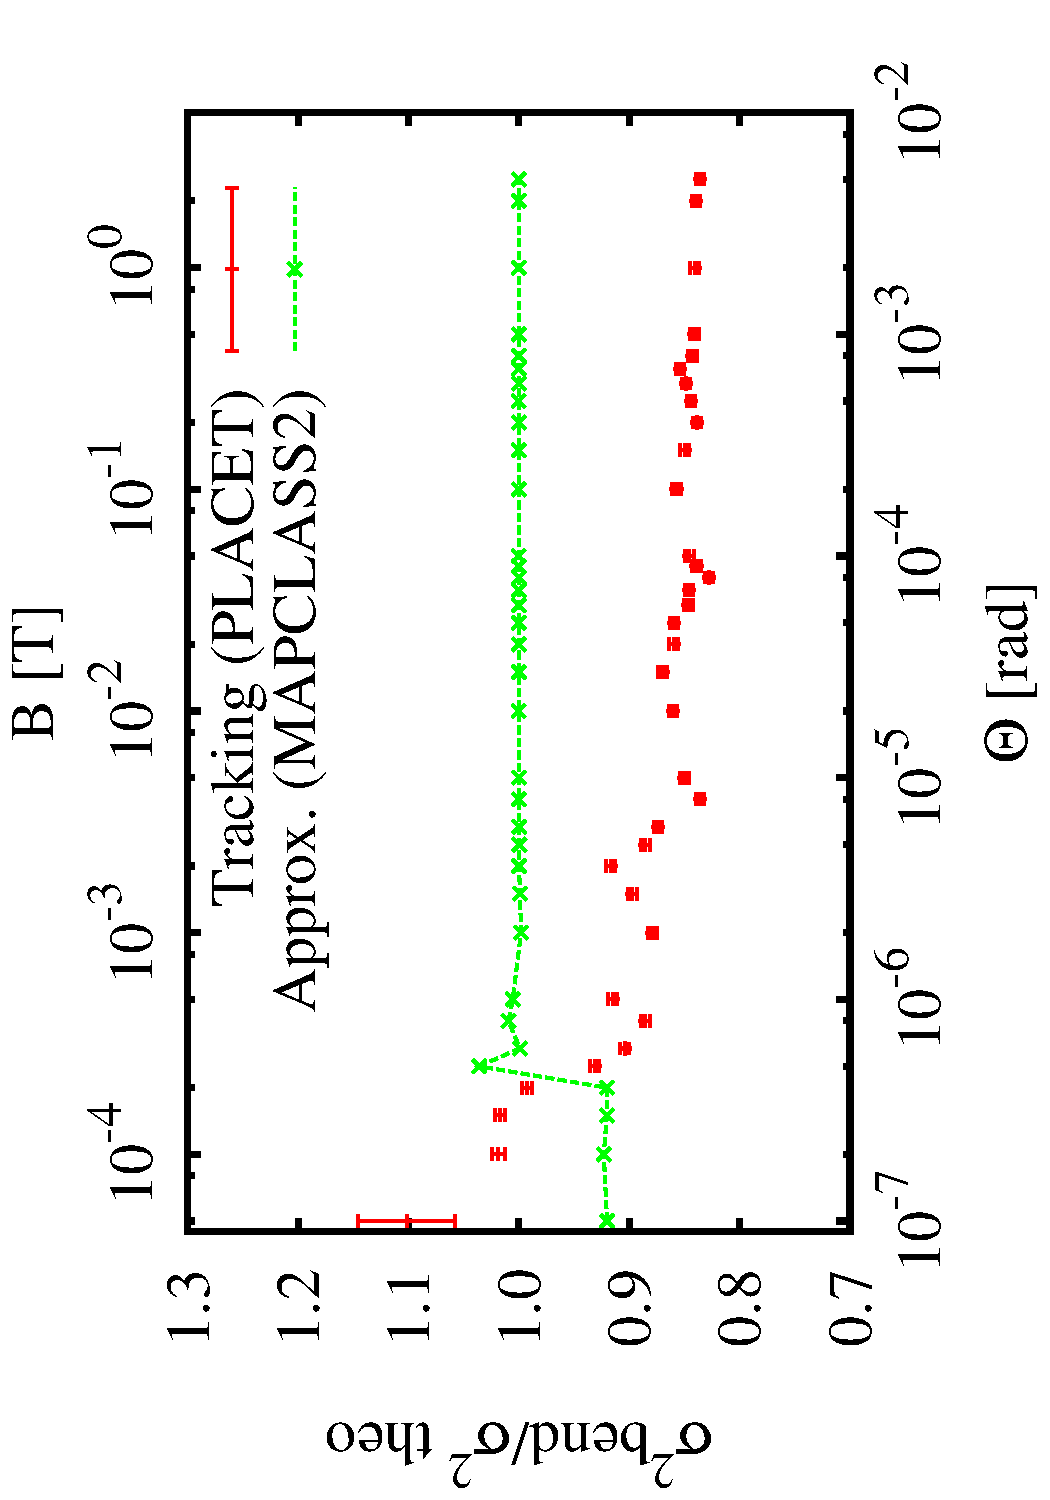
\includegraphics[scale=0.30,angle=-90]{sigma_angle.pdf}
  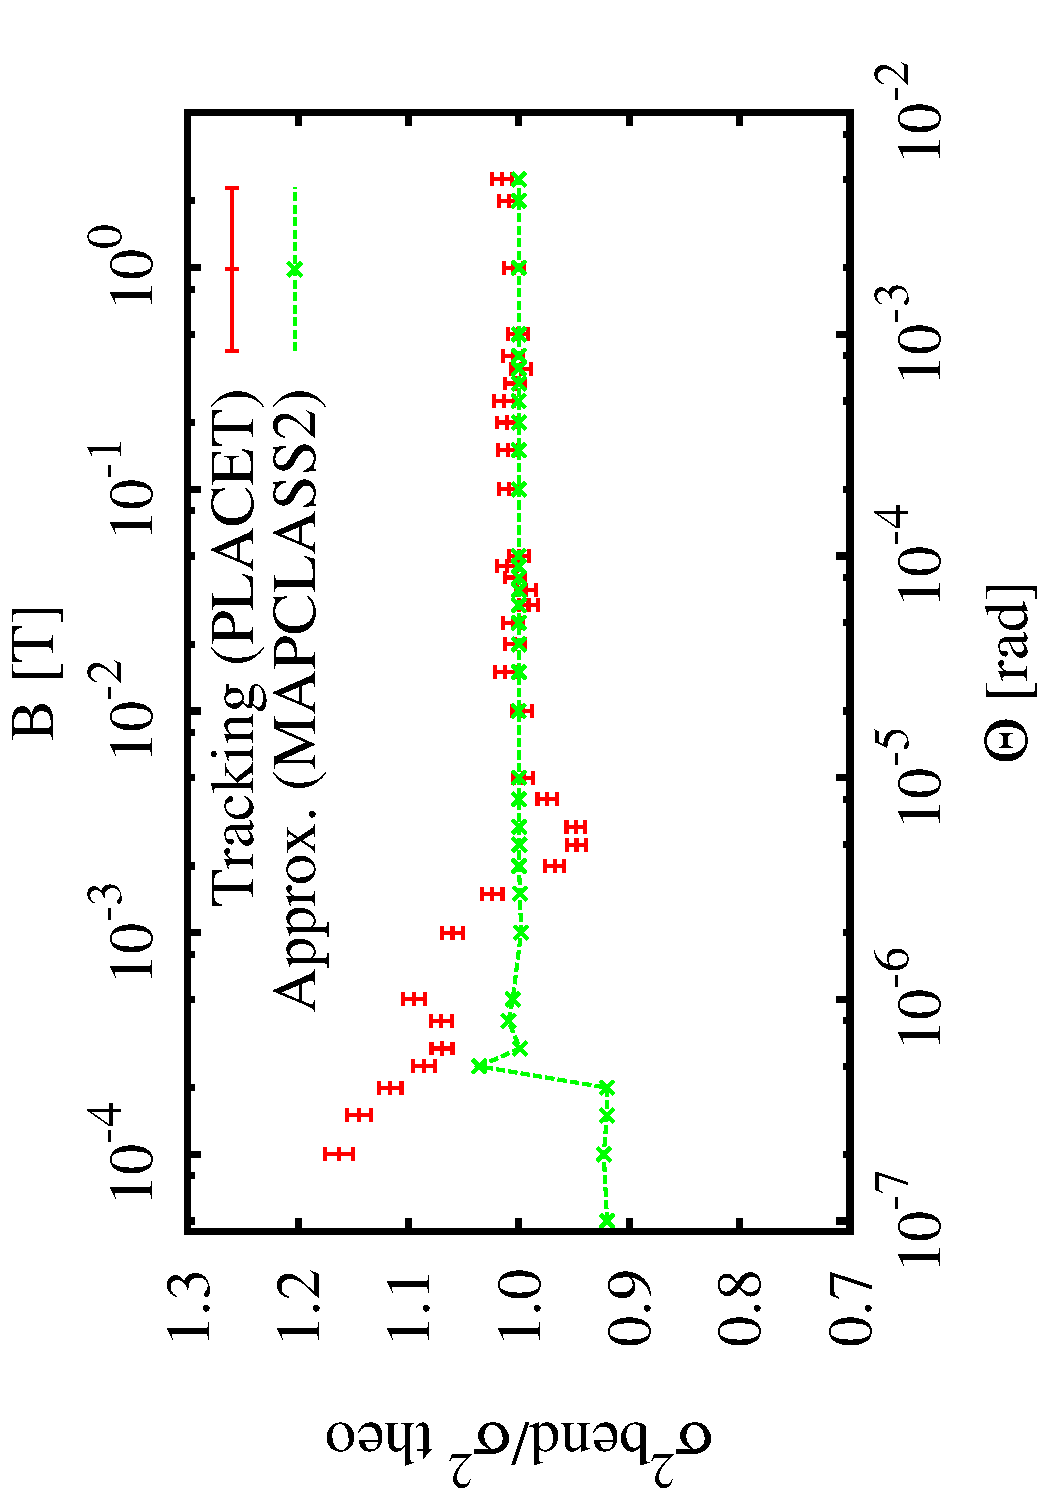
\includegraphics[scale=0.30,angle=-90]{sigma_angle_r06.pdf}\par
%   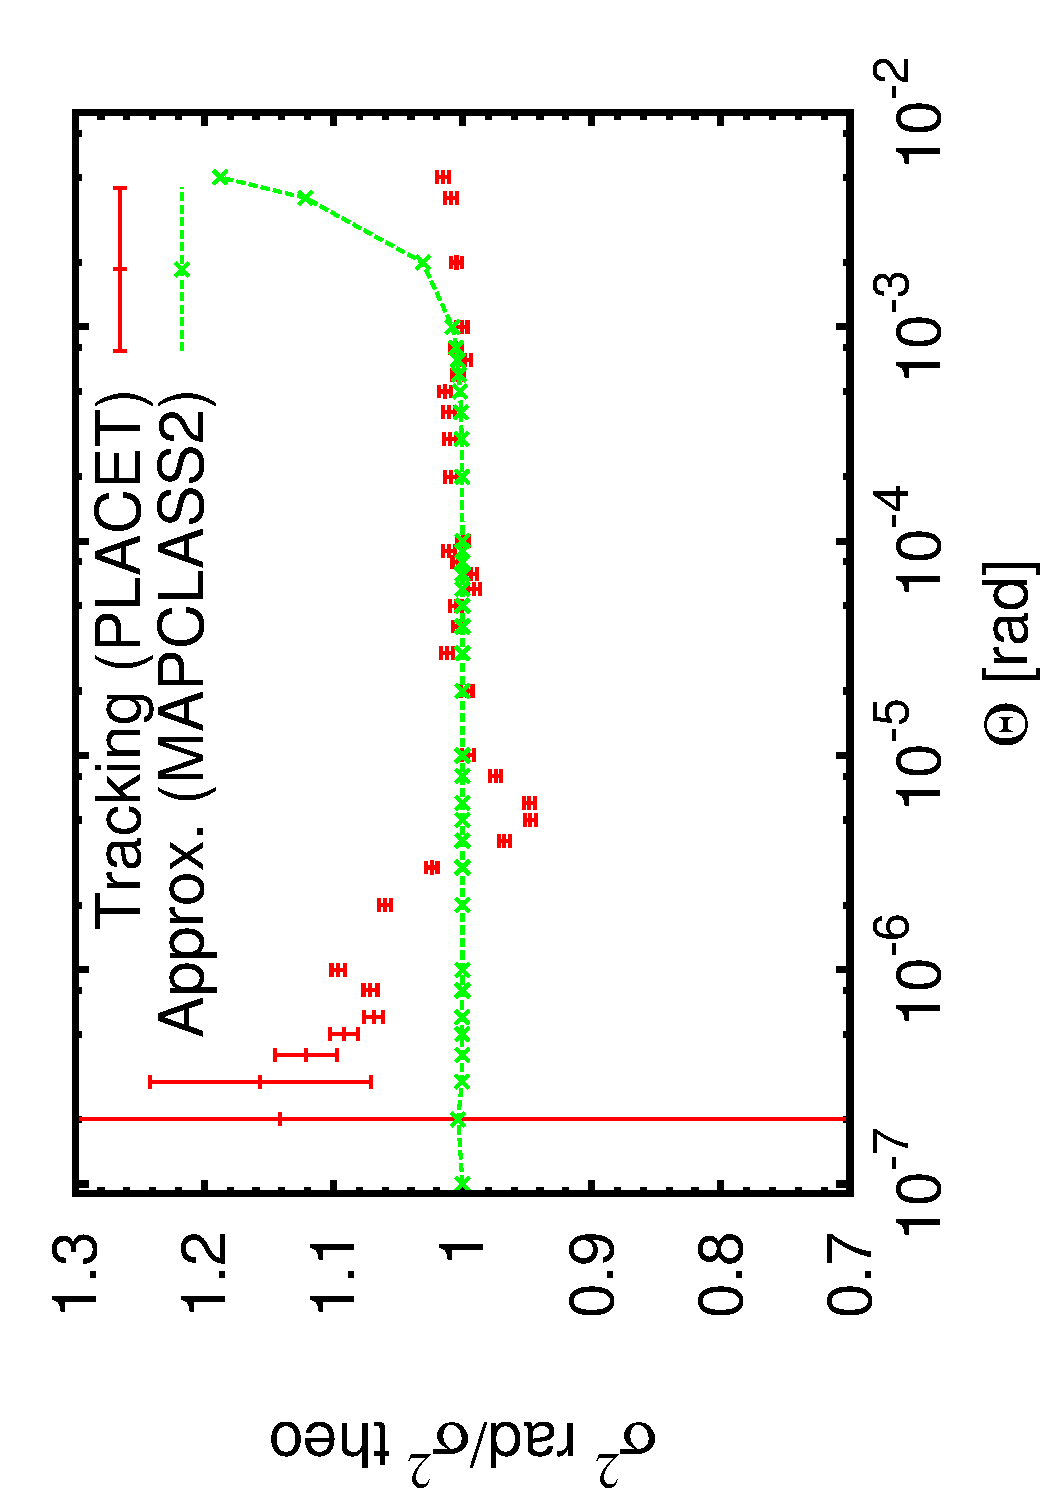
\includegraphics[scale=0.30,angle=-90]{sigma_angle_r6_twiss.pdf}\par
  \hspace*{1.0cm}(a)\hspace*{7.6cm}(b)\par
   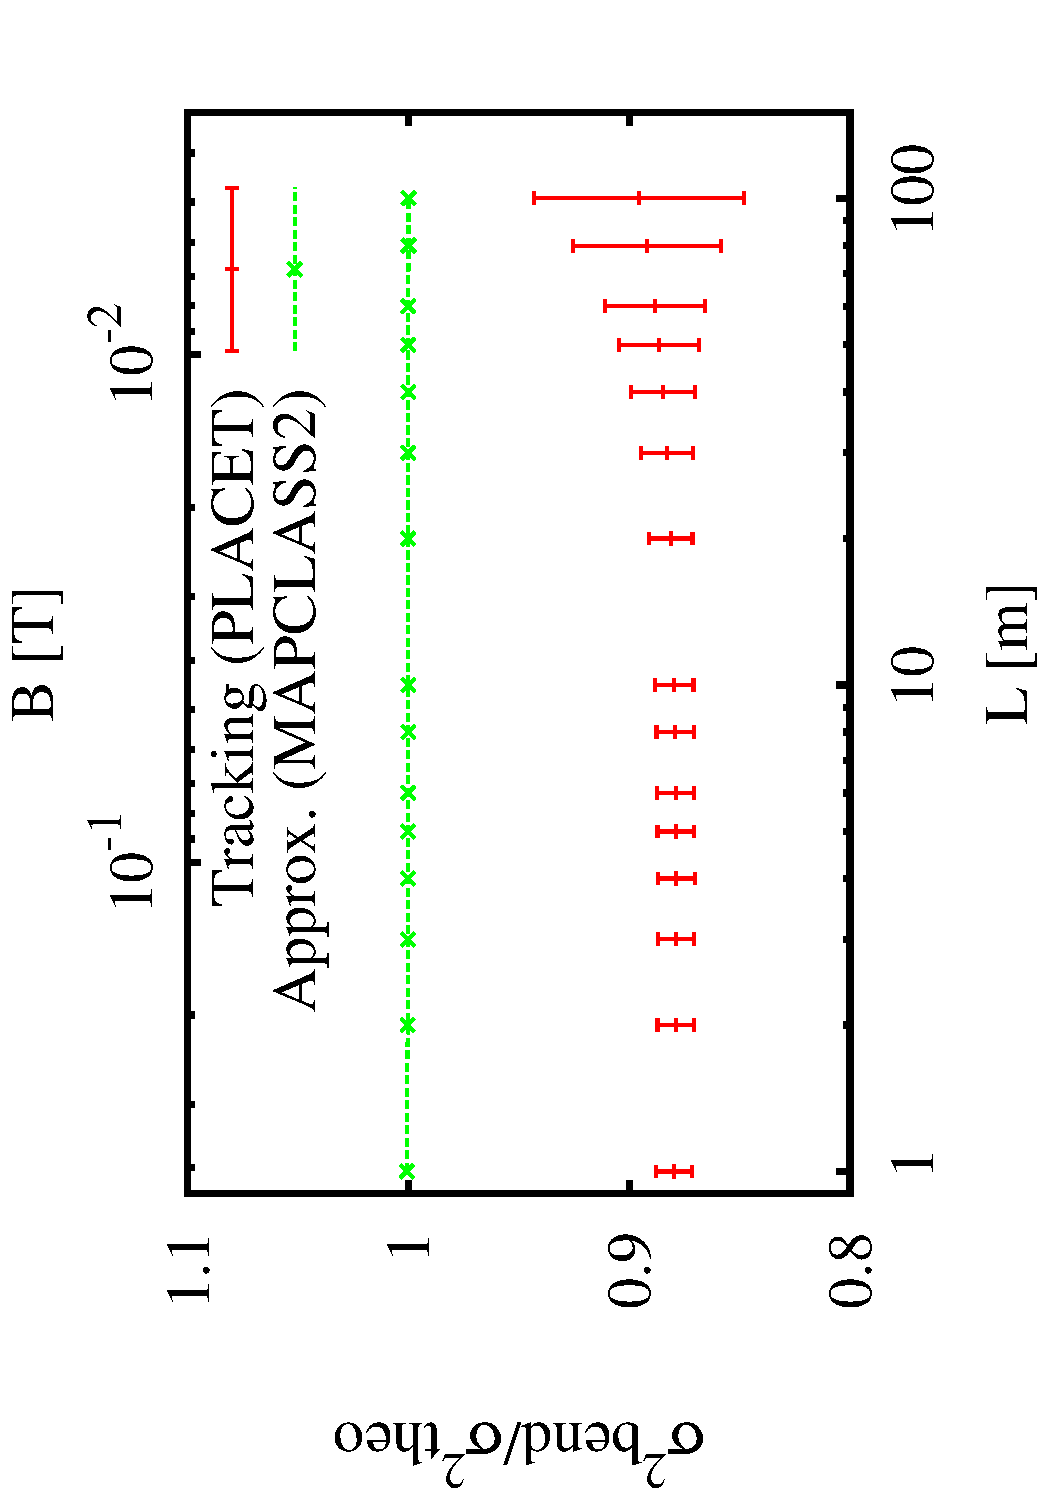
\includegraphics[scale=0.30,angle=-90]{sigma_Lbend.pdf}
  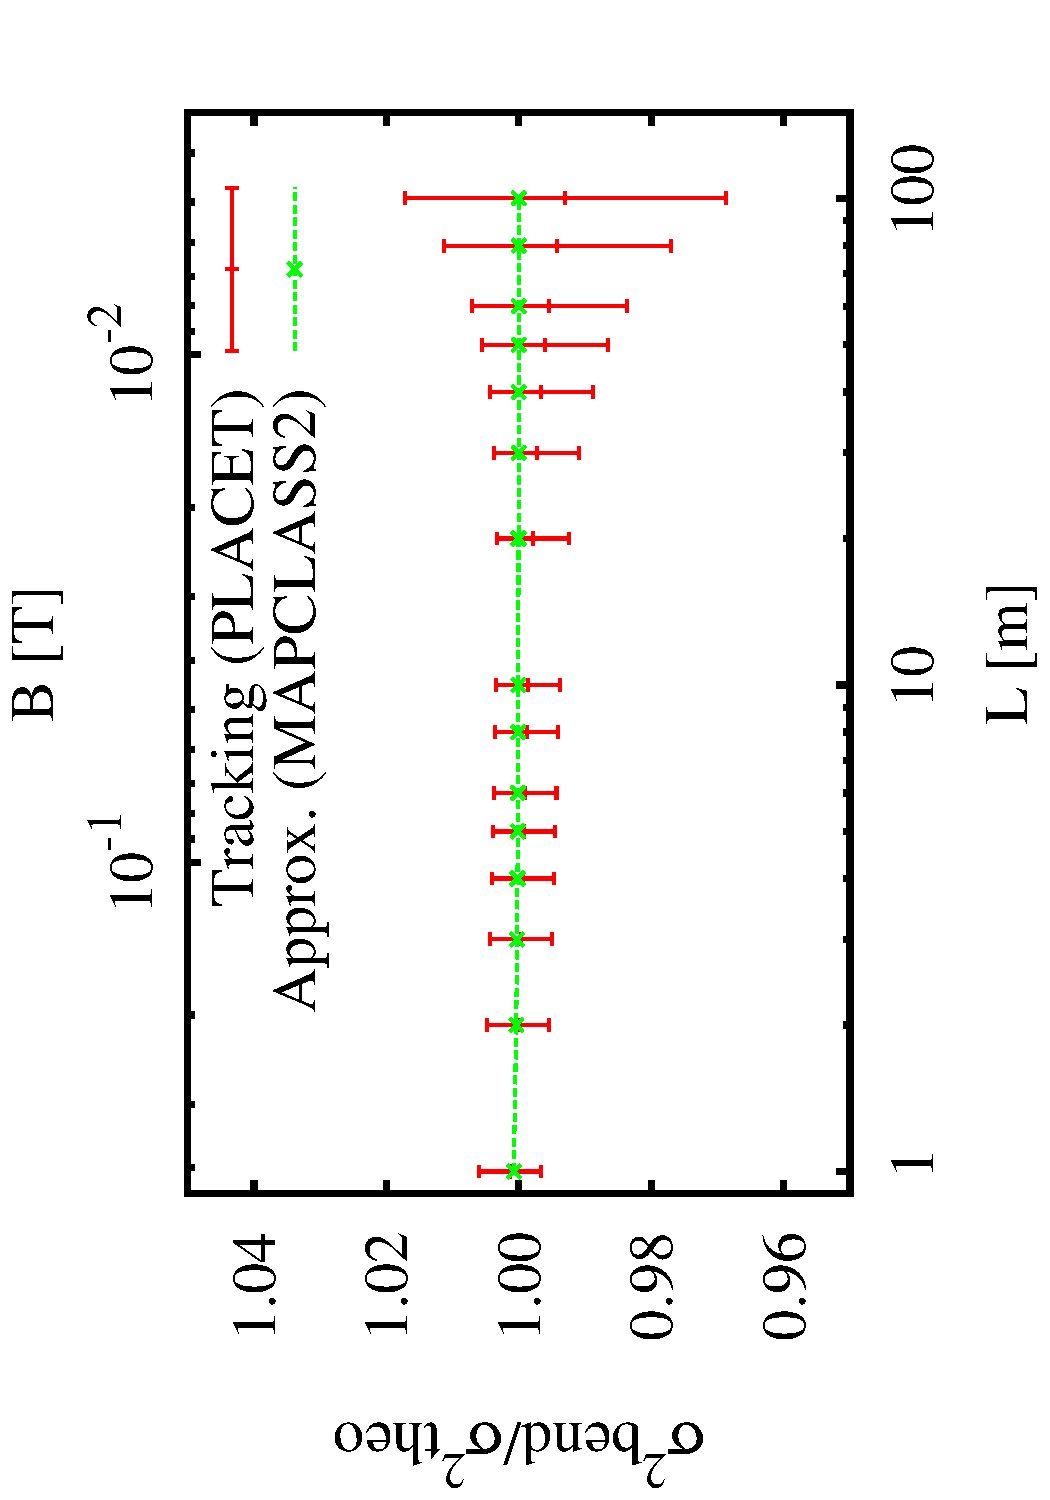
\includegraphics[scale=0.30,angle=-90]{sigma_Lbend_r6.pdf}\par
  \hspace*{1.0cm}(c)\hspace*{7.6cm}(d)\par
  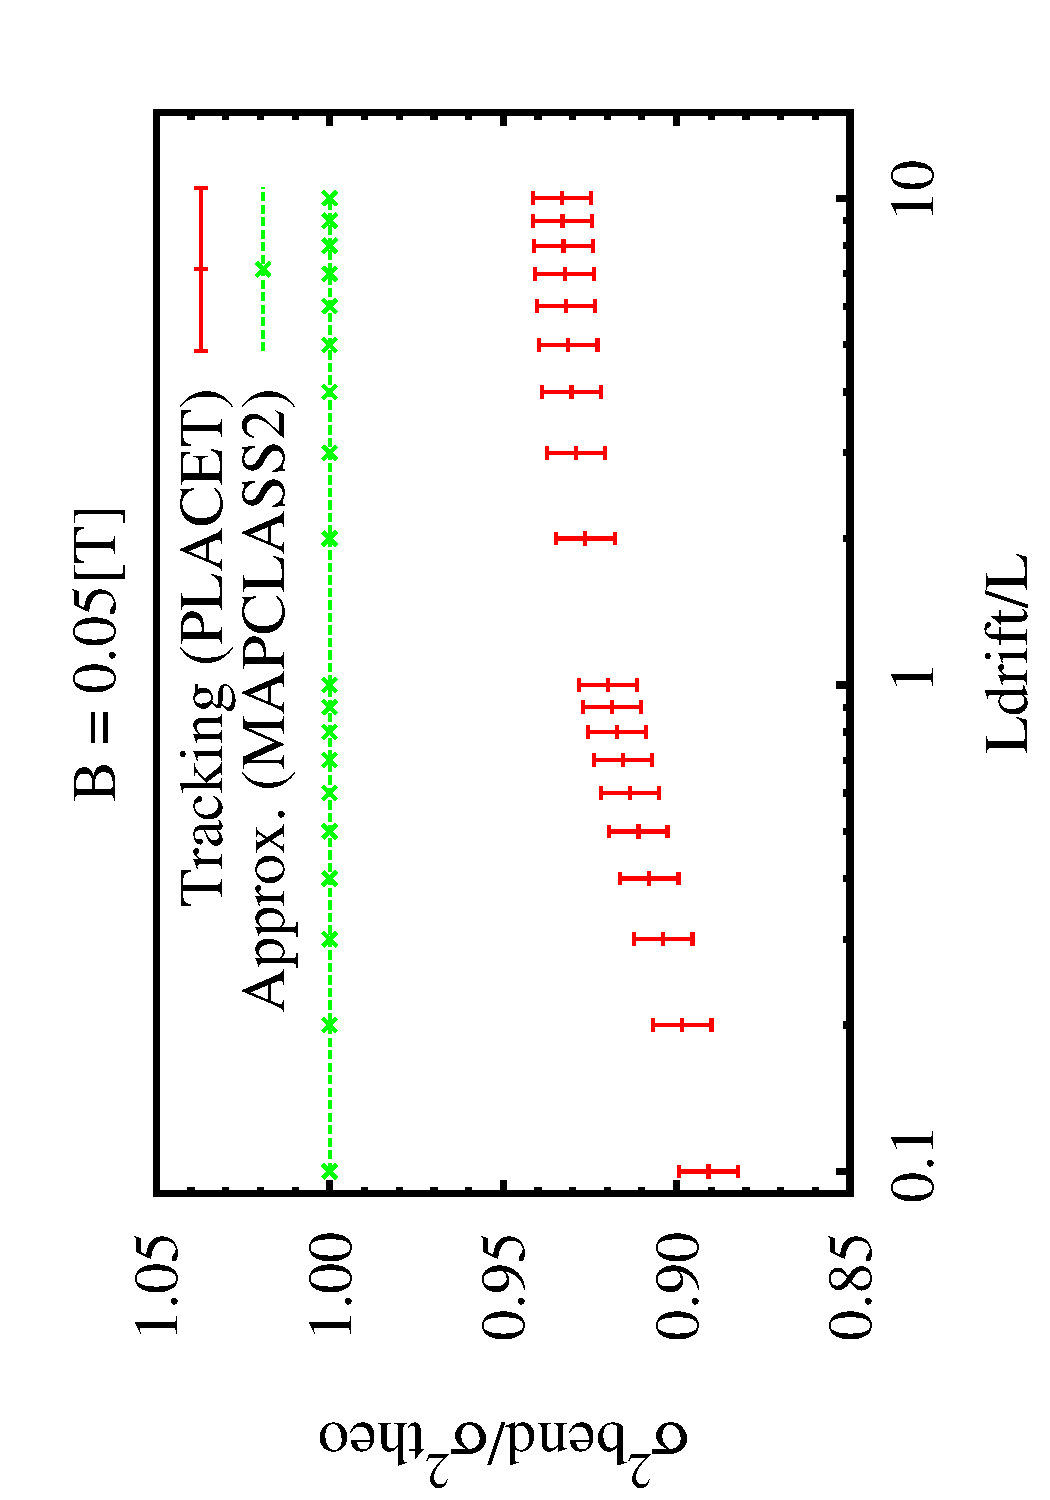
\includegraphics[scale=0.30,angle=-90]{sigma_Ldrift.pdf}
  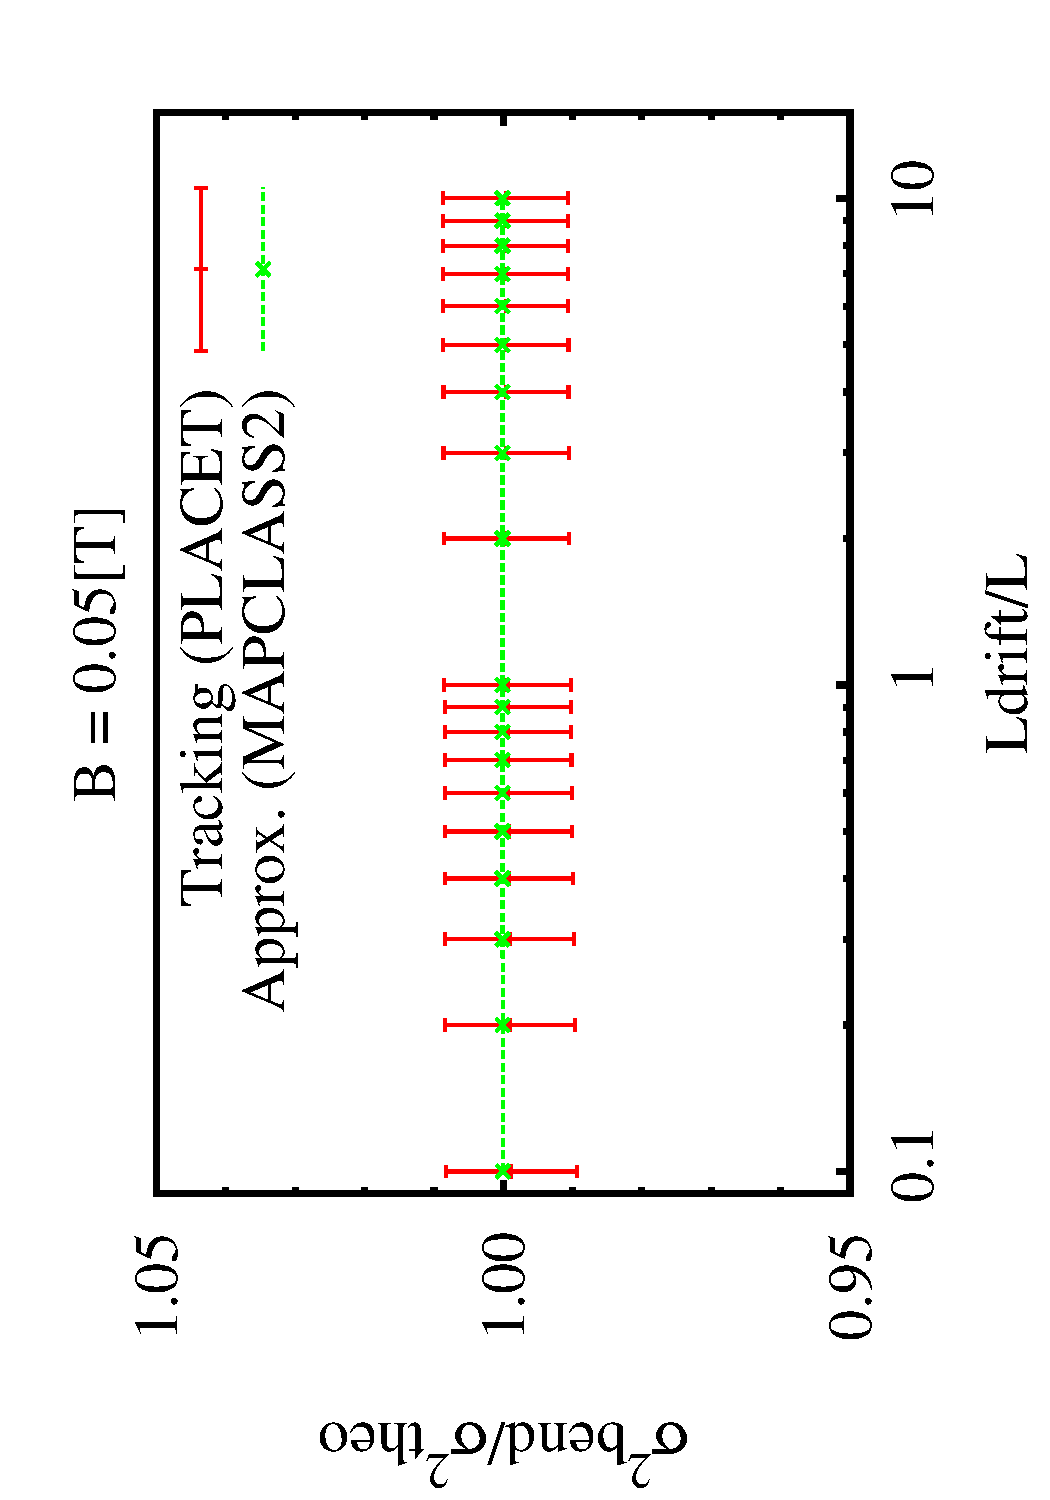
\includegraphics[scale=0.30,angle=-90]{sigma_Ldrift_r6.pdf}
  \hspace*{1.0cm}(e)\hspace*{7.6cm}(f)\par
\caption{Beam size increase due to radiation normalized to theoretical value assuming negligible energy loss. (Left) `Default' radiation option, (Right) `Six\_dim' option in PLACET 0.99.01. Plots (a) and (b) correspond to $L=10$ m for a dipole only. Plots (c) and (d) correspond to $\theta=10^{-4}$ rad for a dipole only. Plots (e) and (f) correspond to $L=10$ m and $\theta=10^{-4}$ rad while varying the drift length. Beam energy is 1500 GeV in all cases.}\label{figSR}
\end{figure}
\clearpage
\section{Model limitations}\label{s:modellim}
The radiation model reviewed is valid when the average number of photons radiated per particle $\langle N\rangle$ is enough to characterize the overall effect in position by its second moment, where $\langle N\rangle  = C_1E\theta$ with $C_1=20.61\text{ GeV}^{-1}$.\par
Although, Sect. \ref{s:comparison} explores the variation of $\theta$, it also changes the magnetic field strength $B$. Here, the magnetic field has been fixed $5 \times 10^{-3}$ T and the magnet length $L$ is systematically shorten to reduce the average number of photons emitted by each particle, equivalent to change $\theta$ because $B\rho$ is fixed for $E=1500$ GeV.\par
Fig. (\ref{figPhotons}) shows how the average number of photons emitted decreases with the dipole length $L$. It is visible also that the region where average is below one photon is also the starting point when tracking and theory start to differ, reaching $\pm10\%$ max.\par
This result is equivalent to the thin dipole approximation mentioned in Sect. \ref{s:comparison}, where the dipole sectioning makes of each slice a binomial trial of photon emission, approaching the Poisson theoretical distribution for large number of slices.\par
\begin{figure}[htb]
\centering
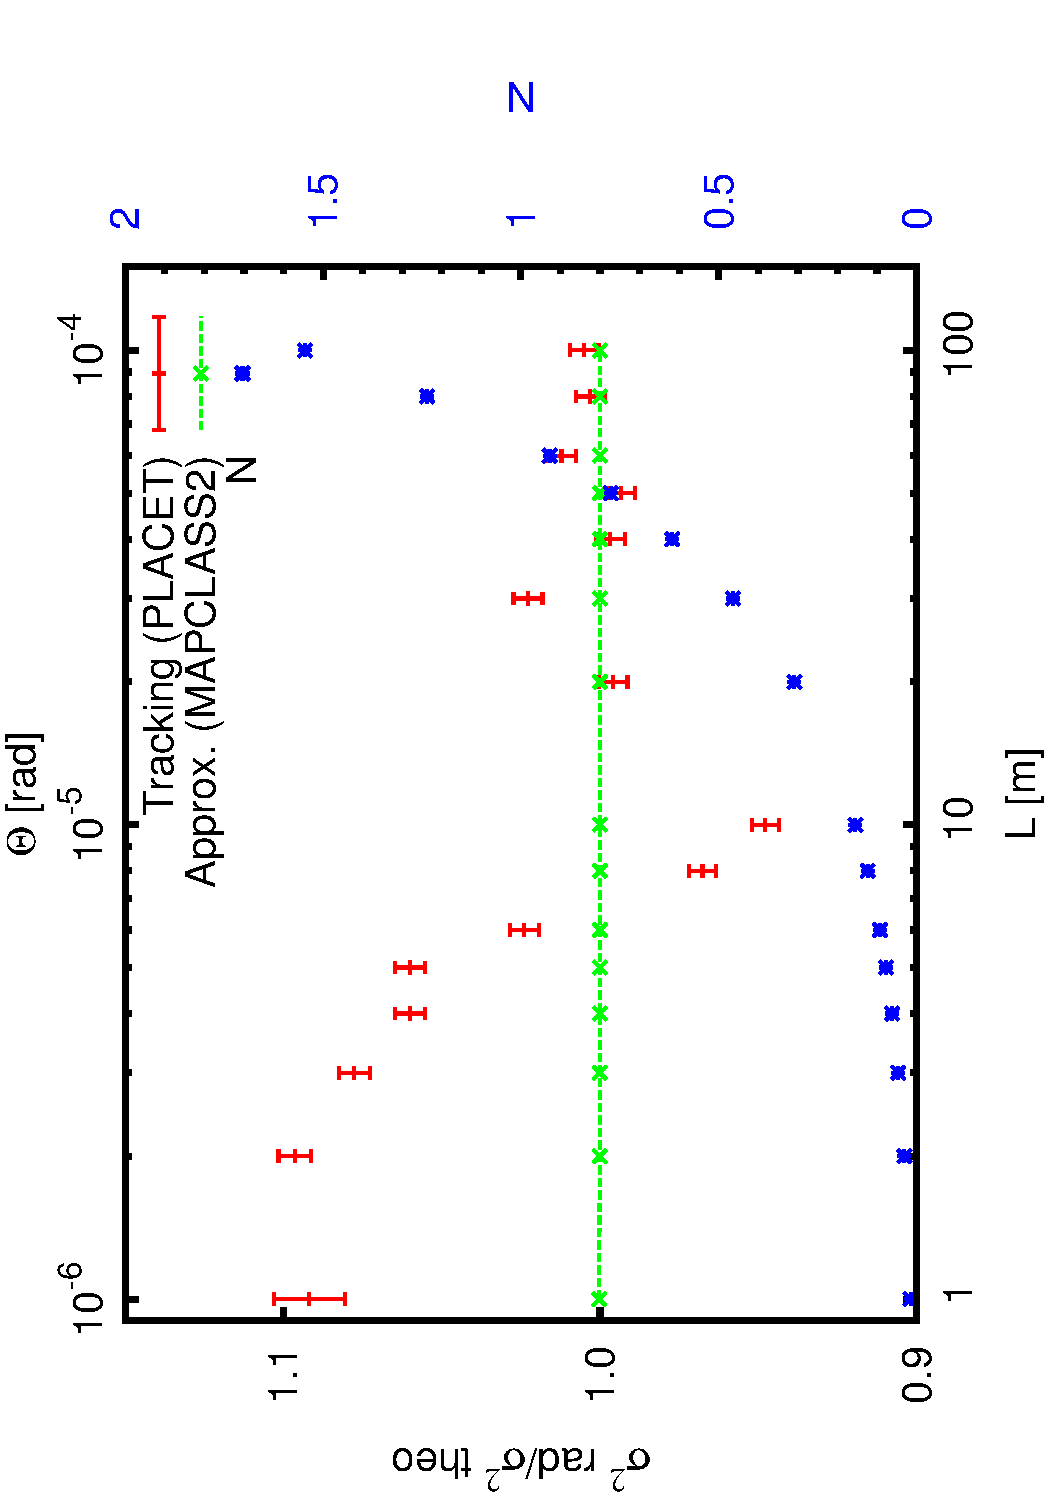
\includegraphics[scale=0.6,angle=-90]{./sigma_Bfix5e-3T.pdf} \caption{Result from tracking, theoretical calculation with the mean number of photons emitted by particle superimposed. Magnetic field is fixed at $5\times 10^{-3}$ T and $E=1500$  GeV.}\label{figPhotons}
\end{figure}

\section{Validity for the FFS}
The CLIC FFS design is composed by magnets with bending angles shown in Table \ref{T-nphotons_3TeV} for 3 TeV and Table \ref{T-nphotons_500GeV} for 500 GeV.  The third column indicates the quantity of magnets used in each of those sections.\par 
Although the average value of photons emitted per magnet is low, these are grouped in long sections with common bending angle. \begin{table}[ht]
\begin{minipage}[b]{0.45\linewidth}\centering
\begin{tabular}{c|c|c}\hline\hline
 $|\theta|$ & $\langle N \rangle$&Qty.\\
 ($\mu$rad)&&\\\hline
 $\;\;$1.1& 0.07 &70 \\
 $\;\;$3.9& 0.24 &20 \\
 17.2& 1.06 &10\\\hline
\end{tabular}\caption{Bending angles in CLIC 3 TeV.}\label{T-nphotons_3TeV}
\end{minipage}
\hspace{0.5cm}
\begin{minipage}[b]{0.45\linewidth}
\centering
\begin{tabular}{c|c|c}\hline\hline
 $|\theta|$& $\langle N \rangle$&Qty.\\
 ($\mu$rad)&&\\\hline
 $\;\;\;\;$8.3& 0.08&70\\
 $\;\;$27.5& 0.28 &20\\
 135.0& 1.39 &10\\\hline
\end{tabular}\caption{Bending angles in CLIC 500 GeV.}\label{T-nphotons_500GeV}
\end{minipage}
\end{table}
Using the conclusions from Sect. \ref{s:modellim} it will be similar to the thin dipole approximation and therefore the expression for beam size contribution from radiation in bending magnets should be within $\pm10\%$ agreement with tracking codes, making it useful for initial lattice optimization.\par

\chapter{Oide effect}
\chapter{Oide effect}
This part of the document addresses the radiation phenomenon in quadrupoles called Oide effect\cite{Oide}, which sets a limit on the beam size demagnification, specially important in linear colliders because of the strong focusing required in the Final Doublet before the Interation Point (IP).\par
First, a brief introduction to the beam size limit (Oide limit) is given, where calculations have been derived to include this radiation phenomenon in the lattice design and optimization software. The Oide effect is evaluated for the CLIC 3 TeV and CLIC 500 GeV parameters, leading to change the length of the first quadrupole before the IP, called QD0. It ends with a proposal to mitigate the impact of the Oide effect by adding correctors before and after the QD0, reducing the beam size.\par
\section{Beam size limit}\label{Oideeffect}
The Oide effect is caused by the interaction of charged particles with the magnetic field from quadrupoles. Radiation in a focusing magnet, schematically represented as QD0 in Fig. (\ref{f:Oideeffect}), changes the energy of the particle and modifies the focusing effect. This results in a limit on the minimum beam size specially relevant in the vertical plane.\par%For the horizontal direction, is mainly affected by radiation caused by the interaction of charged particles with the magnetic field from dipoles. %This report will be limited to sector dipoles or ``sbends''.\par
\begin{figure}[!hbt]
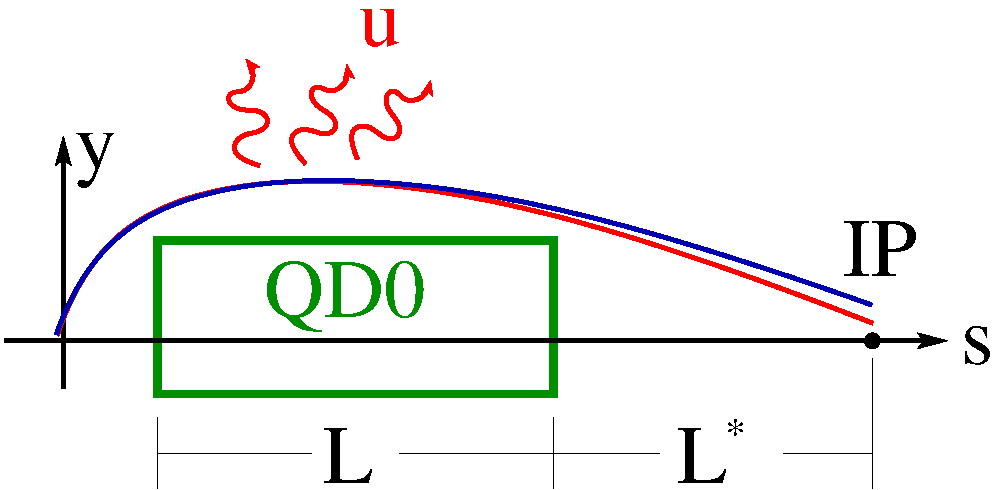
\includegraphics[scale=0.5]{Oide.pdf}
\centering
\caption{Design particle trajectory in blue and the trajectory of a particle due to radiation in the quadrupole in red.}\label{f:Oideeffect}
\end{figure}
 The beam size growth due to radiation is added quadratically to the linear beam size $\sigma_0^2=\epsilon\beta$ where $\beta$ represents the optical beta function and $\epsilon$ is the emittance. Therefore, $ \sigma^2 = \sigma_0^2 + \sigma_{oide}^2$, where the beam size contribution from the Oide effect is \cite{Oide},
 \begin{equation}
  \sigma^2_{oide} = \frac{110}{3\sqrt{6\pi}}r_e\frac{\lambda_e}{2\pi}\gamma^5 F(\sqrt{k}L,\sqrt{k}L^*)\left(\frac{\epsilon}{\beta^*}\right)^{5/2}
  \label{Oideequ}
 \end{equation}
 where
 \begin{equation}
  F(\sqrt{k}L, \sqrt{k}L^*) = \int_0^{\sqrt{k}L}|\sin\phi+\sqrt{k}L^*\cos\phi|^3\left[\int_0^\phi(\sin\phi'+\sqrt{k}L^*\cos\phi')^2 d\phi'\right]^2d\phi
  \label{OideF}
 \end{equation}
  and $\lambda_e$ is the Compton wavelength of the electron, $r_e$ is the classical electron radius, $\gamma$ is the relativistic factor, $\epsilon$ is the geometrical beam emittance, $\beta^*$ is the Twiss parameter at the observation point (in this case, the IP), and $k$, $L$ and $L^*$ are the quadrupole gradient, the quadrupole length and the distance to the observation point measured from the closest magnet face.\par
   Although the total contribution to beam size depends on the lattice and beam parameters, the minimum achievable beam size is given by \cite{Oide}
%the function $F$ is calculated only from quadrupole parameters. For this reason, $F$ will be used as figure of merit for a quadrupole.
\begin{equation}
 \sigma_{y \text{ min}} = \left(\frac{7}{5}\right)^\frac{1}{2}\left[\frac{275}{3\sqrt{6\pi}}r_e\frac{\lambda_e}{2\pi}F(\sqrt{K}L,\sqrt{K}L^*)\right]^\frac{1}{7}(\epsilon_{Ny})^\frac{5}{7}
\end{equation}
where $\epsilon_N=\gamma\epsilon$ is the normalized emittance, showing the independence from beam energy.\par
The only possibility to reduce the beam size is by changing the value of $F$, by modifying the magnet parameters, or to minimize the beam emittance. However, using the ILC 500 GeV \cite{ILCdes}, CLIC 500 GeV and CLIC 3 TeV \cite{CLICdes} parameters, it is possible to conclude from columns $\sigma_0$ and $\sigma_{oide}$ in Table (\ref{t:Sigmas}) that the contribution of the Oide effect to beam size is only significant for CLIC 3 TeV.\par
In addition, columns $\sigma$ and $\sigma_{min}$ in Table (\ref{t:Sigmas}) show that both CLIC designs are close to the minimum achievable beam size.\par
\begin{table}[!hbt]
\centering
{\scriptsize
\begin{tabular}{l||c|c|c||c|c|c|c|c||c|c}\hline\hline
Lattice &$\epsilon_N$& $\gamma$& $\sigma_0$&$k$&$L$&$L^*$& $F$ & $\sigma_{oide}$&$\sigma$&$\sigma_{min}$\\
 &(nm)&($10^3$)&(nm)&(m$^{-2}$)&(m)&(m)&&(nm) &(nm)&(nm)\\\hline
CLIC 3 TeV & 20 & 2935.0 & 0.70 & 0.116 & 2.73 &3.5&  4.086  & 0.85 & 1.10& 1.00 \\
CLIC 500 GeV & 25 & $\;\;$489.2 & 2.3 & 0.077 & 3.35 &4.3& 4.115 & 0.08 & 2.3 & 1.17\\
ILC  500 GeV & 40 & $\;\;$489.2 & 5.7 & 0.170 & 2.20 &4.3& 9.567 & 0.04 & 5.7 & 1.85\\\hline
\end{tabular}\caption{Vertical beam size and radiation beam size contribution for three lattices. $\epsilon_N$ is the normalized emittance, $\epsilon_N=\gamma\epsilon$.}\label{t:Sigmas}
}
\end{table}

\section{Oide Double Integral Solution}\label{s:DoubleIntegral}
In this section the double integral used to calculate $F$ is solved with the goal to increase the computational calculation speed. It was included in MapClass2\cite{Mapclassorig,Mapclass,Mapclass2,githubMapClass2} to be used in lattice design and optimization.\par
  The inner integral over $\phi'$ can be solved because it has a known primitive.
\begin{equation}
 \int_0^\phi (\sin \phi'+ \sqrt{k}l^*\cos\phi')^2d\phi'=\frac{\phi}{2}[(\sqrt{k}l^*)^2 +1 ] + \frac{\sin(2\phi)}{4}[(\sqrt{k}l^*)^2 -1]+\sqrt{k}l^*\sin^2\phi
\end{equation}
The Eq. (\ref{OideF}) can now be expressed as one integral.
{\scriptsize
\begin{align}
F(\sqrt{k}L&,\sqrt{k}l^*) =\\
&\int_0^{ \sqrt{k}L} |\sin\phi+\sqrt{k}l^*\cos\phi|^3 \left( \frac{\phi}{2}[(\sqrt{k}l^*)^2 +1 ] + \frac{\sin(2\phi)}{4}[(\sqrt{k}l^*)^2 -1]+\sqrt{k}l^*\sin^2\phi\right)^2 d\phi\notag
\end{align}
}
The squared factor in brackets is always positive because all inner terms are real. The term inside the absolute value is also always positive, therefore, the integrand is always positive. Now, considering the function:
  \begin{equation}
  |\sin \phi + \sqrt{k}l^*\cos\phi|=\left\{
  \begin{array}{c l l}
&  \sin\phi+\sqrt{k}l^*\cos	\phi,\quad\qquad&\text{if}, \sin\phi+	\sqrt{k}l^*\cos	\phi\geq0\\
&  -(\sin\phi+\sqrt{k}l^*\cos\phi),\quad&\text{if}, \sin\phi+	\sqrt{k}l^*\cos	\phi<0
  \end{array}\right.\label{eq-absval}
 \end{equation}
sign changes at every point $\quad\phi_n = \arctan(-\sqrt{ k}l^*)\pm n\pi,\quad n\geq1$.\par
It is possible to split the integration interval $i$ times, being $i$ the number of $\phi_n$ solutions where $0<\phi_n<\sqrt{k}L$. On each of those intervals, the absolute value definition can be removed and replaced by the corresponding expression in Eq. (\ref{eq-absval}), having only a difference in sign. By defining the primitive $\mathscr{F}$ in an interval where the factor inside the absolute value is positive it is possible to evaluate $F$ as it is shown in Eq. (\ref{eq-primeval}).
\begin{equation}
 F(\sqrt{k}L,\sqrt{k}l^*)= \mathscr{F}|_0^{\phi_1} - \mathscr{F}|_{\phi_1}^{\phi_2} +  \mathscr{F}|_{\phi_2}^{\phi_3} - \mathscr{F}|_{\phi_3}^{\phi_4}+ \cdots \pm  \mathscr{F}|_{\phi_i}^{\sqrt{k}L}\label{eq-primeval}
\end{equation}
The change of signs in each interval is only  given by the absolute value definition, then, it is simpler to add the absolute value of each contribution.
\begin{equation}
 F(\sqrt{k}L,\sqrt{k}l^*)= \bigr\vert\mathscr{F}|_0^{\phi_1}\bigr\vert + \bigr\vert\mathscr{F}|_{\phi_1}^{\phi_2}\bigr\vert +  \bigr\vert\mathscr{F}|_{\phi_2}^{\phi_3}\bigr\vert + \bigr\vert\mathscr{F}|_{\phi_3}^{\phi_4}\bigr\vert + \cdots +\bigr\vert\mathscr{F}|_{\phi_i}^{\sqrt{k}L}\bigr\vert
\end{equation}
If we know the primitive $\mathscr{F}$ and we are able to calculate the $\phi_n$s in the integration interval, then, it is possible to calculate the factor $F$ without using an approximate integrator. The double integration has been simplified to a primitive evaluation.\par
The primitive $\mathscr{F}$ exists and it has been calculated using Maxima \cite{Maxima} and Wolfram Alpha Mathematica\cite{Wolfram} software, the expression is in Appendix \ref{c:primitiveF}.\par
  
 
\section{Mitigating the impact on the beam size}
\subsection{QD0 length}
As shown in Sect. \ref{Oideeffect} the Oide beam size contribution depends on a combination of beam and optics parameters. %Table \ref{tabSigmas} gives the results.
If none of the beam parameters is to be changed then $F$ can be used as a figure of merit of the optics as it is calculated only from $k$, $L$ and $l^*$. The target is to reduce it as much as possible. Two energy cases are analyzed in the following: 3 TeV ($l^*=3.5$ m) and 500 GeV ($l^*=4.3$ m).\par
Columns $\sigma_0$, $\sigma_{oide}$ and $F$ in Table \ref{t:Sigmas} show that CLIC 3 TeV and 500 GeV \cite{CLICdes,TomasCLIC} have larger contributions to beam size even having a lower $F$ value than ILC 500 GeV \cite{ILCdes}.\par
In order to evaluate the minimum possible $F$ for $l^*$ given, the minimum $k$ required to get the particles focused is when the Twiss function $\alpha$ is zero just at the quadrupole opposite face to the IP.\par
Figure \ref{fig-3TeV:a}  shows the ratio squared between the beam size contribution due to Oide effect and the linear beam size for three cases: when $k$ is the minimum required to get particles focused (to get $\alpha_y=0$ at QD0 opposite side to the IP), when $k$ is calculated as thin lens ($k=\frac{1}{Ll^*}$), and the current QD0 status. Fig. \ref{fig-3TeV:b} shows the $k$ values for the previous mentioned cases.\par
The Oide contribution to beam size is of the same order of the linear beam size. It might be possible to reduce it by doubling the current quad length and using a lower $k$ between the minimum required for the focusing and the thin lens approximation. This also points to increasing the lattice length as this change reduces the tolerance to variations of $\alpha$ at the quadrupole input.\par
Quad lengths larger than 10 m do not lead to further improvements with the current parameters.\par

\begin{figure}[!htb]
\centering
\hspace*{-0.6cm}
\begin{subfigure}{0.45\textwidth}
\centering
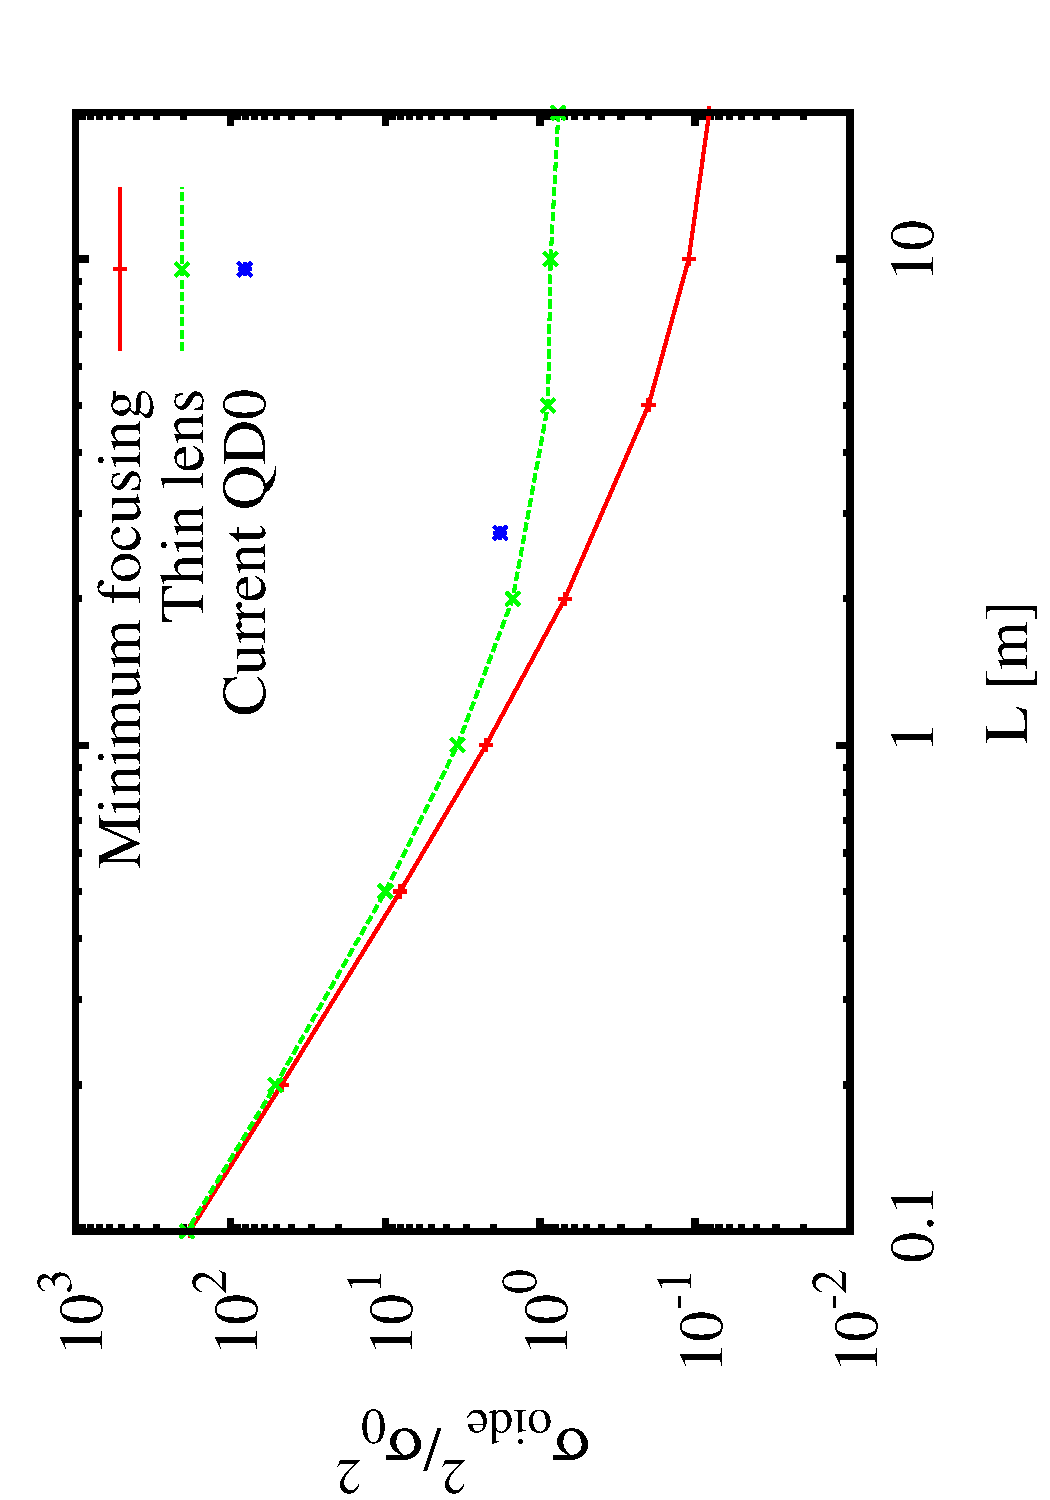
\includegraphics[scale=0.3,angle=-90]{image07a.pdf}\caption{}\label{fig-3TeV:a}
\end{subfigure}
\begin{subfigure}{0.45\textwidth}
\centering
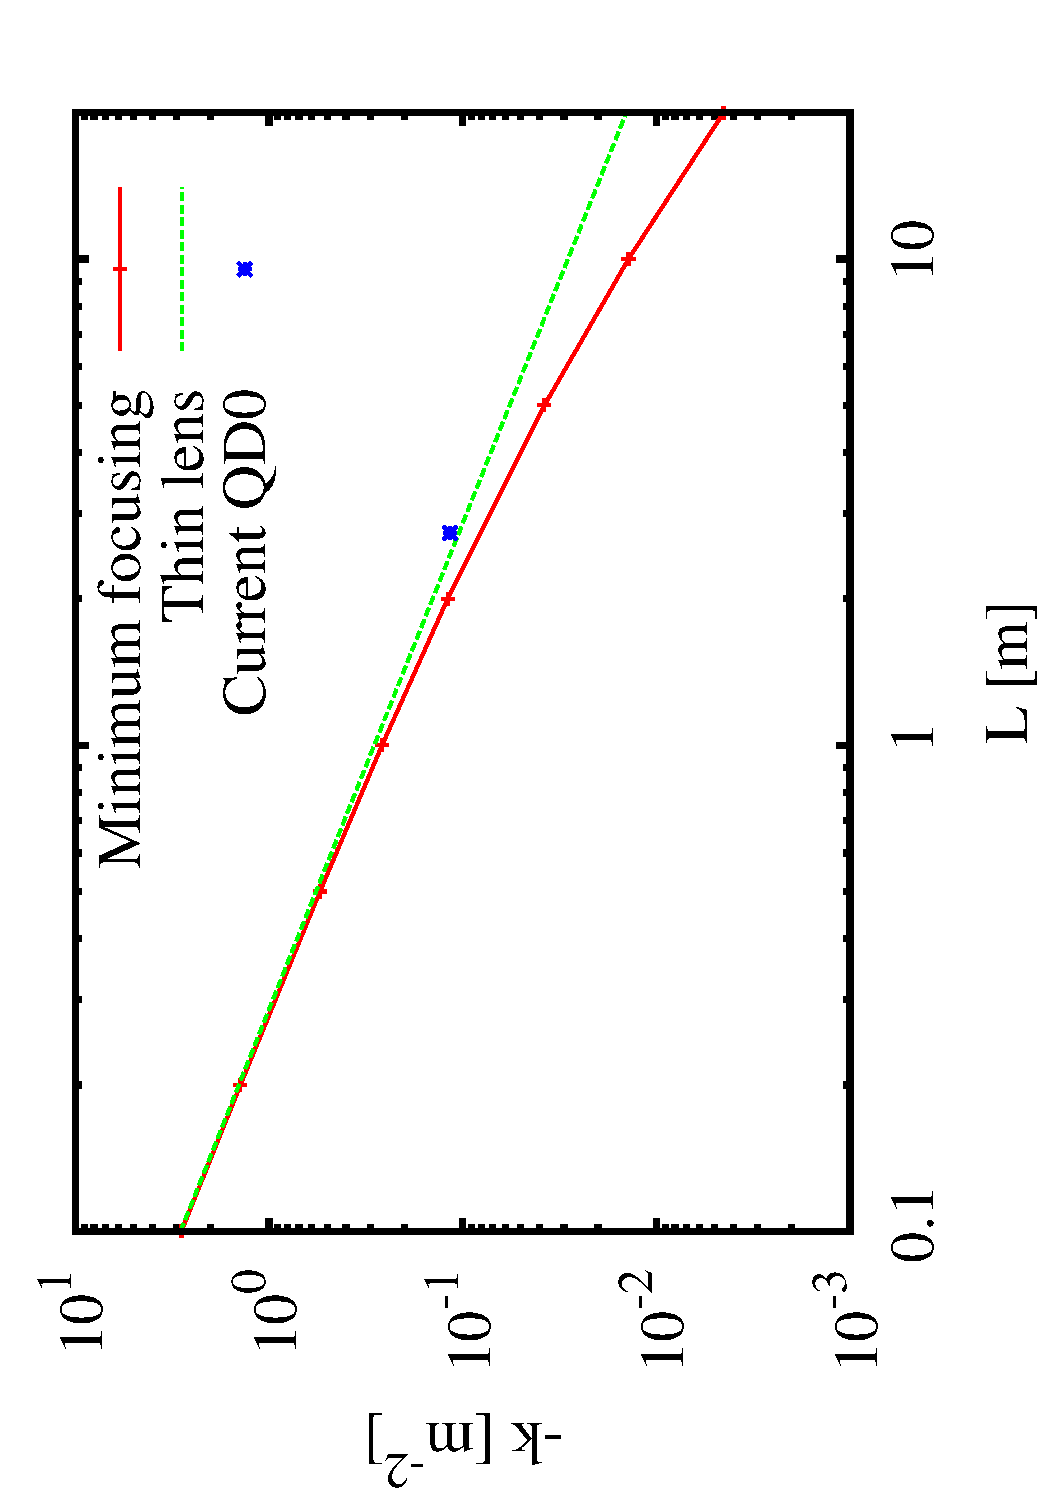
\includegraphics[scale=0.3,angle=-90]{image07b.pdf}\caption{}\label{fig-3TeV:b}
\end{subfigure}
\caption{Oide effect beam size contribution for CLIC 3 TeV design parameters. (a) $\sigma^2_{oide}$ normalized to designed linear beam size as a function of quad length for the minimum focusing $k$ (when $\alpha_y=0$ at the quadrupole opposite side to the IP), for $k$ calculated as thin lens ($k=\frac{1}{Ll^*}$) and the current QD0. (b) $k$ in the three previous cases for comparison.}\label{fig-3TeV}	
 \end{figure}\par
Figure \ref{fig-500GeV} is the corresponding to Fig. \ref{fig-3TeV} for the 500 GeV case. The current design contributes less than 4\% of the total beam size, concluding that the current QD0 length with the CLIC 500 GeV parameters does not need adjustment.\par
\begin{figure}[!htb]
\centering
\hspace*{-0.6cm}
\begin{subfigure}{0.45\textwidth}
\centering
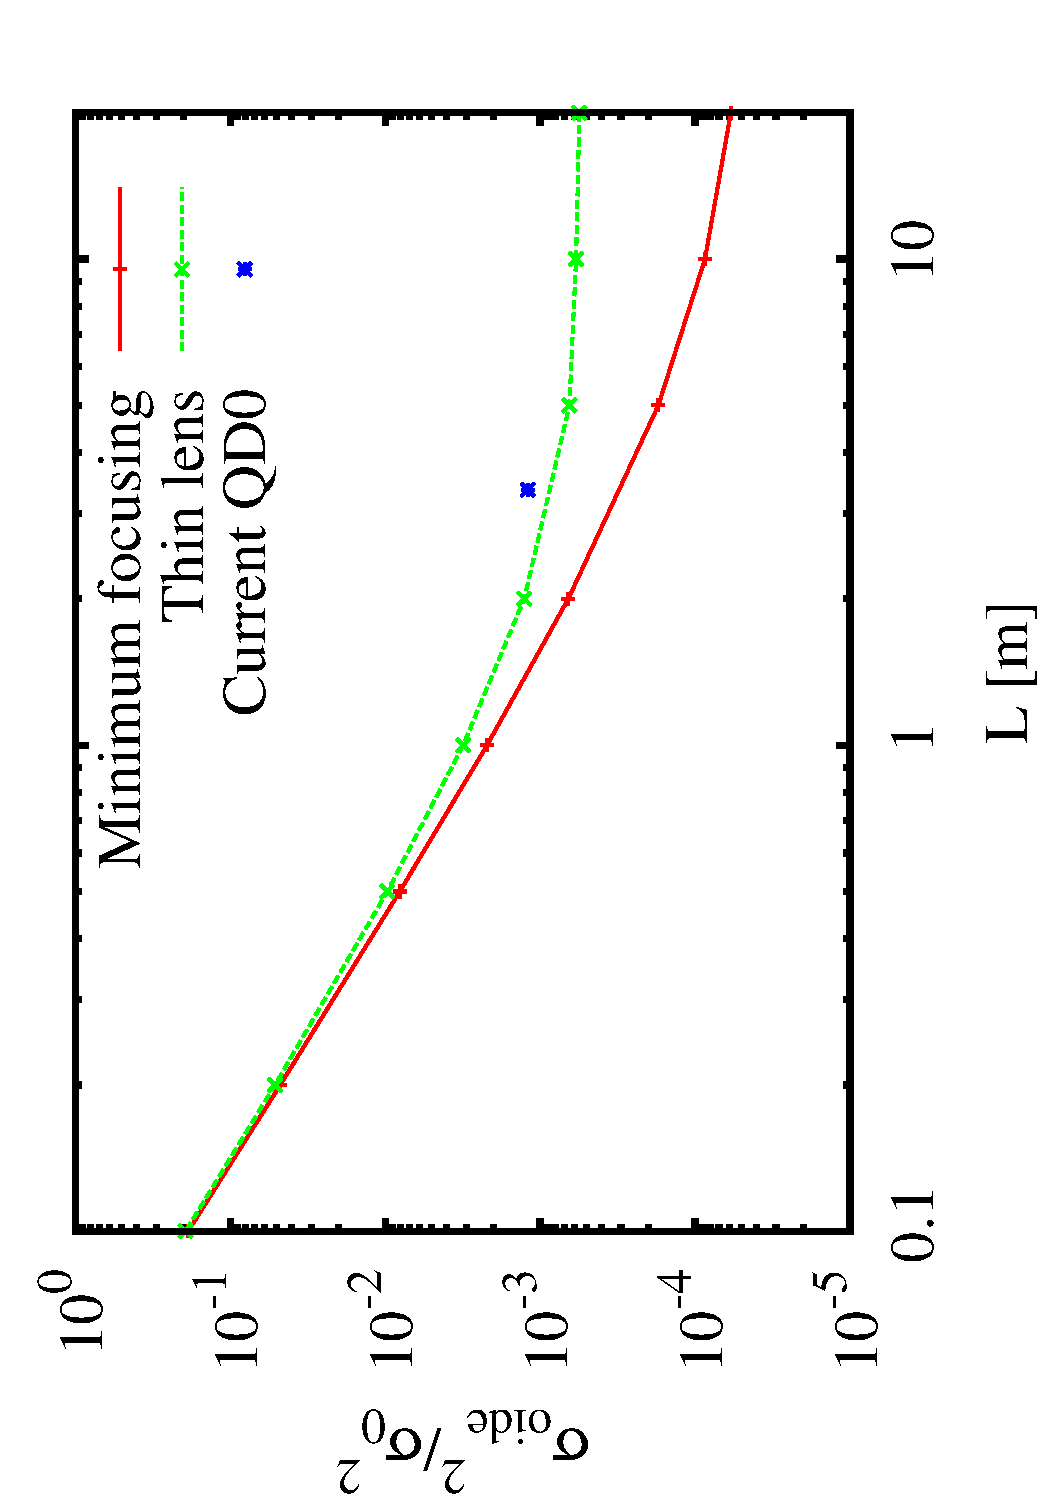
\includegraphics[scale=0.3,angle=-90]{image06b.pdf}\caption{}
\end{subfigure}
\begin{subfigure}{0.45\textwidth}
\centering
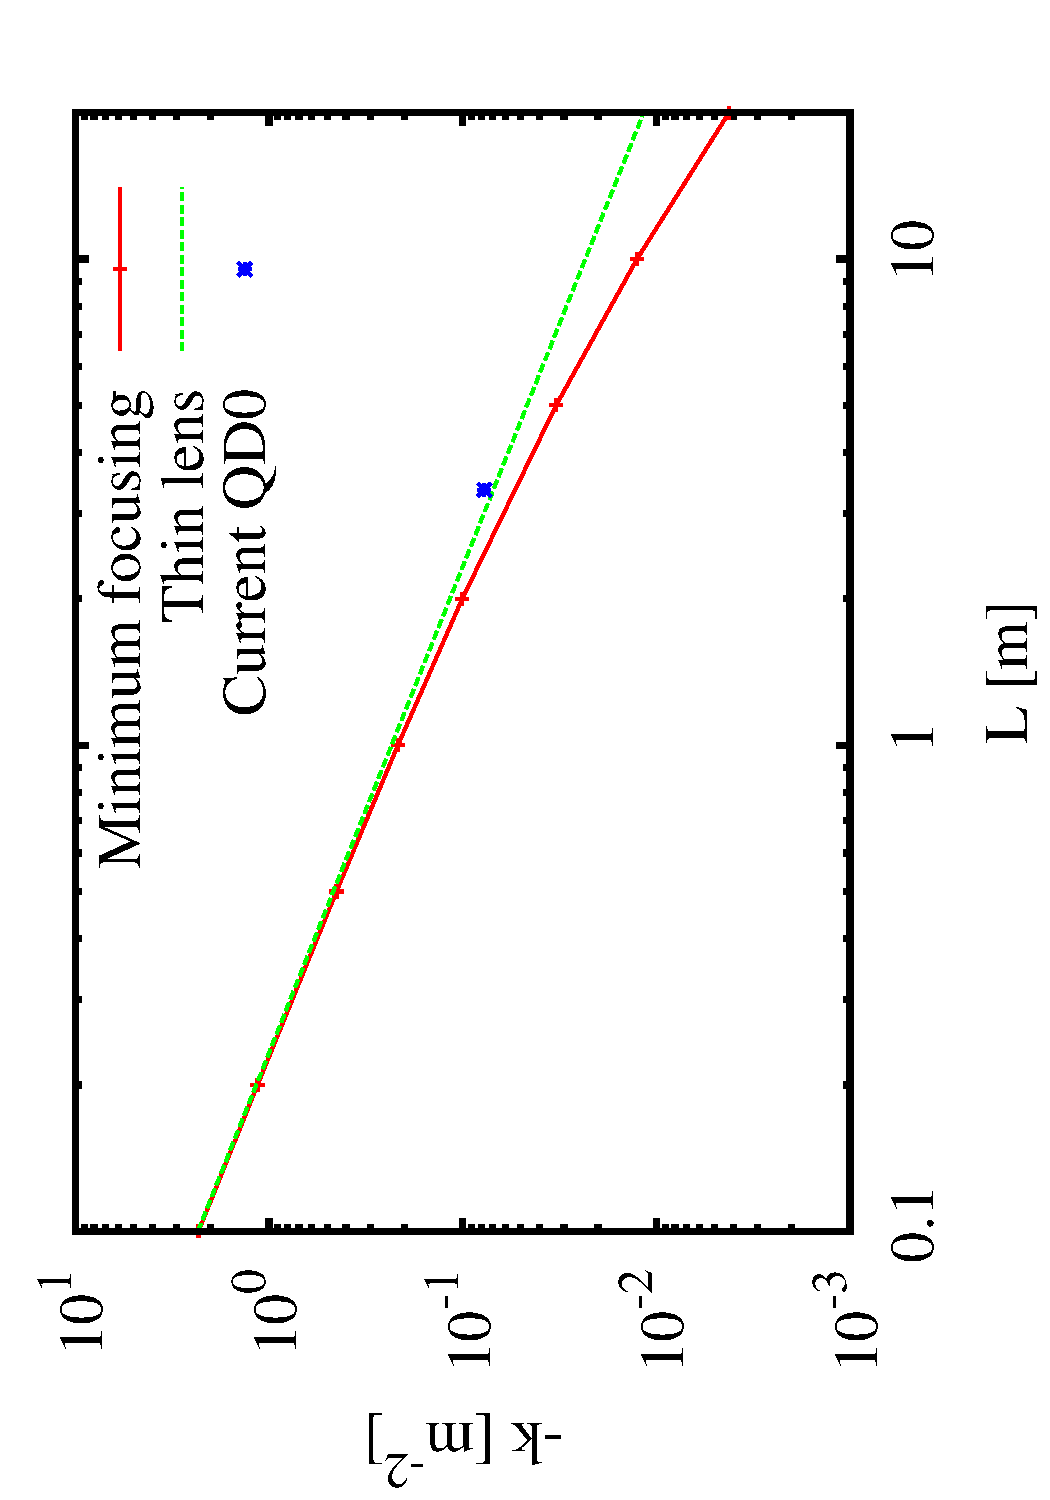
\includegraphics[scale=0.3,angle=-90]{image06c.pdf}\caption{}
\end{subfigure}
\caption{Oide effect beam size contribution for CLIC 500 GeV design parameters. (a) $\sigma^2_{oide}$ normalized to designed linear beam size as a function of quad length for the minimum focusing $k$ (when $\alpha_y=0$ at the quadrupole opposite side to the IP), for $k$ calculated as thin lens ($k=\frac{1}{Ll^*}$) and the current QD0. (b) $k$ in the three previous cases for comparison.}\label{fig-500GeV}
 \end{figure}\par	

\subsection{Correctors}
\subsubsection{$\Delta y$ due to radiation}
Particle tracking from the imput of QD0 to the IP for CLIC 3 TeV with and without radiation, using PLACET \cite{Placet}, allows one to compute the effects of radiation on the six dimentional phase space. Figure \ref{f:CLIC3TeVbeamsizeIP} shows the current transverse distribution of particles at the IP. To compensate the adverse effects a compensation system would ideally remove the position change due to radiation $\Delta y = y_\text{rad} -y_0$.\par
\begin{figure}[!htb]
\centering
 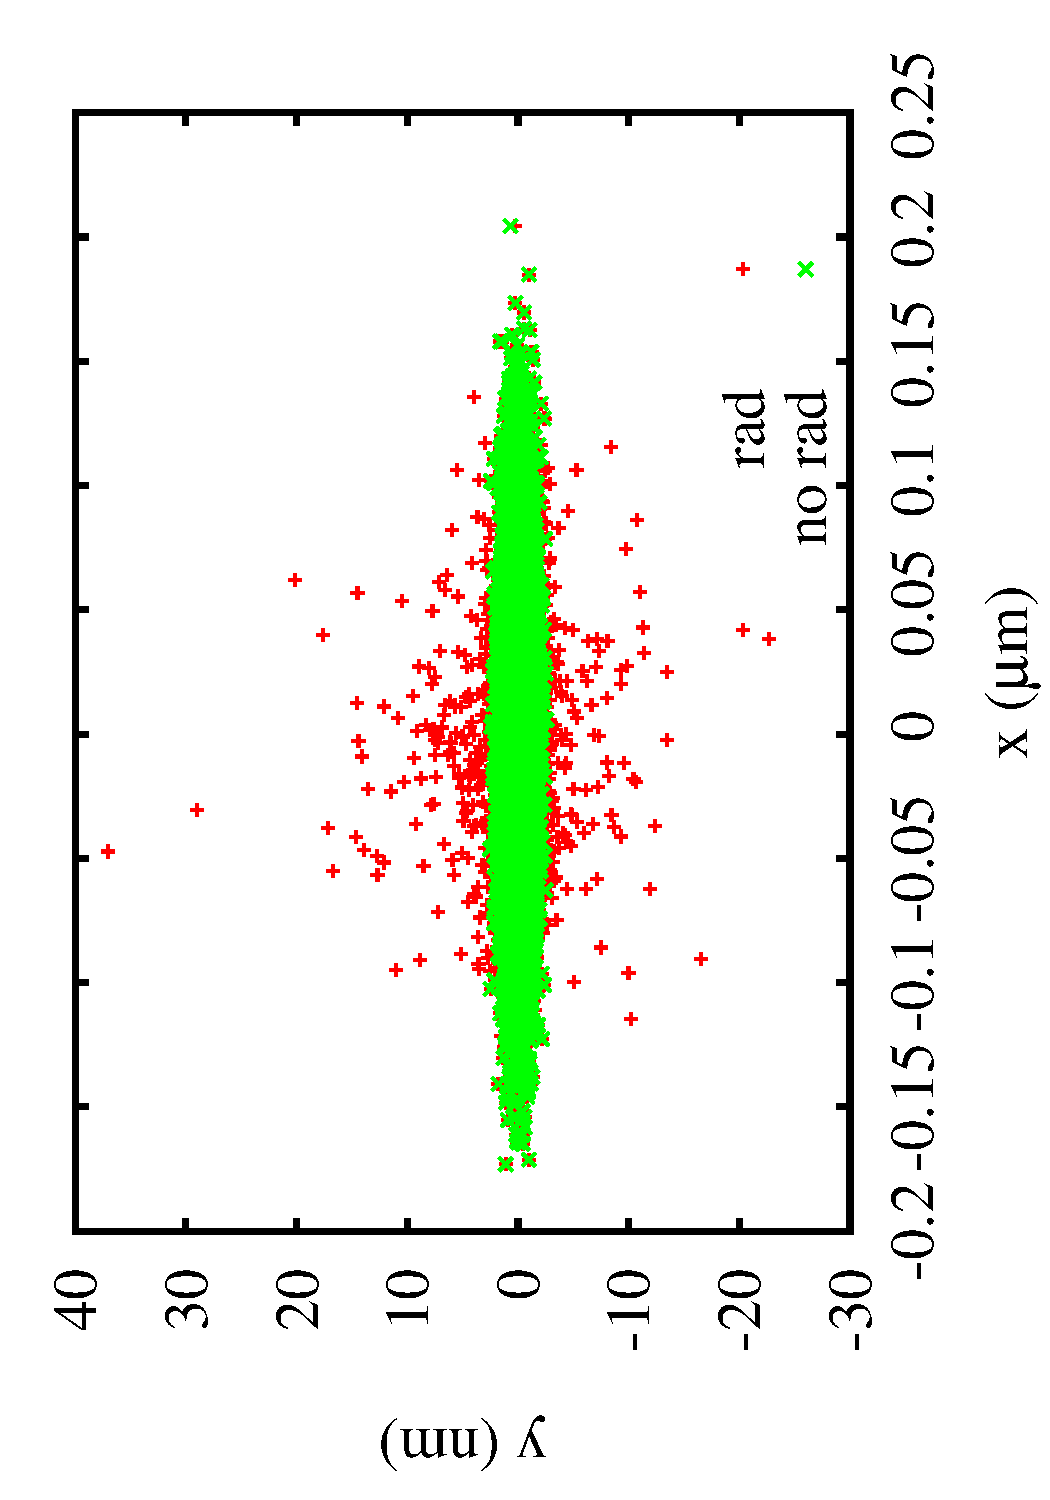
\includegraphics[scale=0.3,angle=-90]{plotxyrad.pdf}\caption{CLIC 3 TeV beam at the IP after tracking through 	QD0 with and without radiation.}\label{f:CLIC3TeVbeamsizeIP}
\end{figure}
Although the average radiation effect is zero, $\langle \Delta y \rangle = 0$ because of the cubic term $(y_0')^3$ as stated by Oide \cite{Oide}, the correlation between $\Delta y, y'$ is not zero. The correlation expression is shown in Eq. (\ref{eq:deltamean}).
\begin{equation}
 \langle\Delta y,y'_0\rangle = \frac{2}{3}r_e\gamma^3G(\sqrt{K}L,\sqrt{K}L^*)(y'_0)^3\label{eq:deltamean}
\end{equation}
%$r_e$ is the clasical electron radius and 
where $G(\sqrt{K}L,\sqrt{K}L^*)$ is given by
\begin{equation}
\int_0^{\sqrt{K}L}(\sin\phi+\sqrt{K}L^*\cos\phi)^2\int_0^\phi (\sin\phi'+\sqrt{K}L^*\cos\phi')^2 d\phi'd\phi
\end{equation}
Fig. \ref{f:correlation} shows the comparison between the correlation obtained from tracking and the theoretical evaluation of the previous expression.\par
\begin{figure}[!htb]
\centering
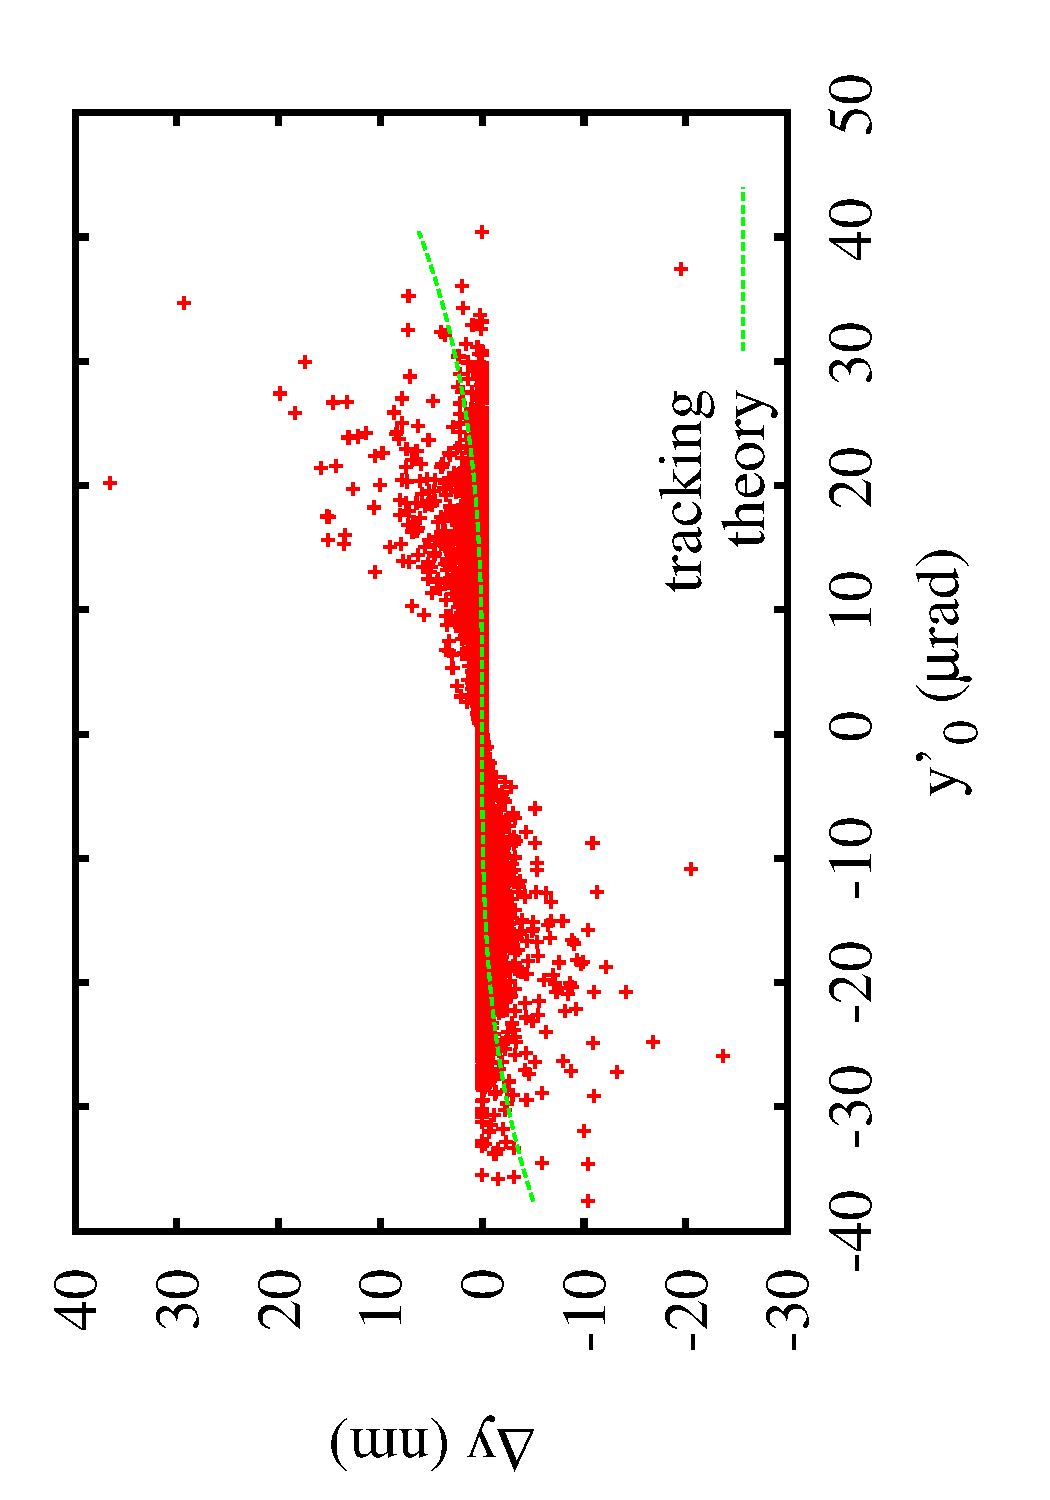
\includegraphics[scale=0.3,angle=-90]{plotdyrad.pdf}\caption{Correlation between the phase space coordinates $\Delta y,y'$ for CLIC 3 TeV from particle tracking and theoretical expression in Eq. (\ref{eq:deltamean}).}\label{f:correlation}
\end{figure}
This correlation could be removed from the beam size by a set of octupolar correctors to be presented in next Section.
\subsubsection{Correctors}
A pair of correctors, placed as in Fig. \ref{f:corrector}, is added to the strong focusing in order to mitigate the radiation effect. Particles that did not radiate along QD0 receive kicks in C1 and C0 cancelling one another. However, the C1 and C0 kicks do not cancel for particles that did radiate, this difference is used to correct only the particles trajectory change due to radiation.\par
The procedure consists in scaning the best position and multipole gradient ($s,k_i$) for C0, and then set C1 at QD0 input to cancel the effect of C0. If two points with same $\beta_y/\beta_x$ ratio are chosen, then the mutual cancellation of C1 and C0 correctors is limited only by the phase advance between them \cite{PhysRevSTAB.8.104002} and angle dispersion in the general case. Figure \ref{f:betaratio} shows the horizontal and vertical $\beta$ functions for CLIC 3 TeV in FD region, and their ratio.\par
The equal $\beta_y/\beta_x$ ratio for C0 and C1 condition is difficult to fulfill because C0 should be too close to the IP. In addition, it will lead to correctors running at very high strengths perturbing the beam.\par
A second approach is to minimize the phase advance between correctors. Therefore they will be located on both faces of QD0. This has the advantage of correctors running at lower strengths thanks to large $\beta$ functions.\par
\begin{figure}[!htb]
\centering
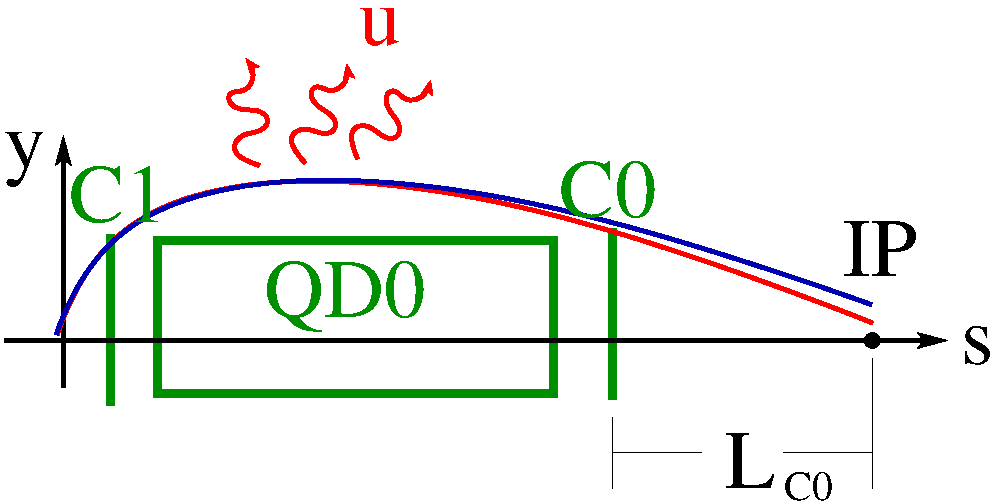
\includegraphics[scale=0.5,angle=0]{Oide2.pdf}\caption{For the nominal trajectory in blue, the kick in C1 must cancel the kick in C0. For all particles that radiate in red, the difference in kicks should cancel $\Delta y$.}\label{f:corrector}
\end{figure}
\begin{figure}[!htb]
\centering
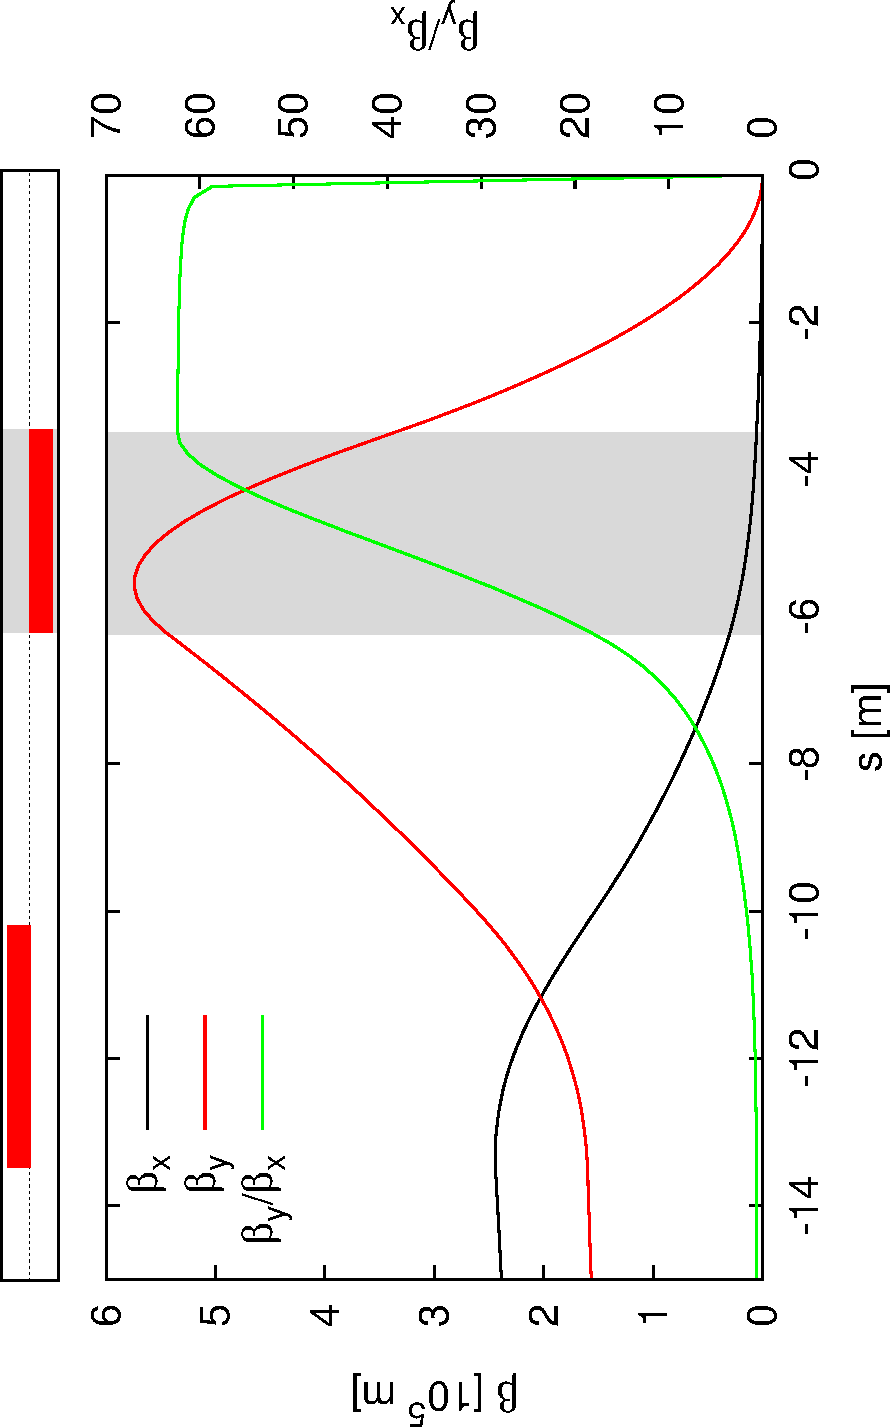
\includegraphics[scale=0.45,angle=-90]{lattice_CLIC_3TeVFD-crop.pdf}\caption{$\beta$ functions and $\beta_y/\beta_x$ ratio for CLIC 3 TeV FD, QF1 and QD0 in red on top. The dark area is occupied by QD0 and the IP is at $s=0$.}\label{f:betaratio}
\end{figure}
Two octupoles (OD0,OD1) were tried as correctors (C0,C1) to substract the cubic fit. A CLIC 3 TeV nominal beam with no energy spread is generated at the IP and tracked back to the entrance of the C1 without radiation with both correctors off. This beam is used to study the Oide effect mitigation in QD0 using correctors by tracking to the IP with radiation.\par
The best result obtained with the octupole correctors is a vertical beam size reduction by $(-4.3\pm0.2)$\% using OD0 only. Table \ref{t:correctors} shows the result of luminosity changes less than 10\% for the case with no radiation in QD0, with radiation, with one corrector and with the two correctors obtained with Guinea Pig ++ \cite{Schulte:382453}.\par
\begin{table}[!hbt]
\centering
\scriptsize
\begin{tabular}{c||c|c|c|c||c|c||c|c}\hline
& \multicolumn{2}{c|}{OD1} &\multicolumn{2}{c||}{OD0} & $\sigma_x$ & $\sigma_y$ & $L_{tot}$ & $L_{peak}$\\
& $L$ [m] & $k_3$ [m$^{-4}$] & $L$ [m] & $k_3$ [m$^{-4}$] &  [nm] & [nm] & \multicolumn{2}{c}{[$10^{34}$cm$^{-2}\cdot s^{-1}$]}\\\hline\hline
NO RAD & 0.01 & 0 & 0.01 & 0 & 47.45 & 0.69 & 7.7 & 2.9\\
RAD    & 0.01 & 0 & 0.01 & 0 & 47.45 & 1.18 & 7.5 & 2.7 \\
RAD    & 0.01 & 0 & 0.01 & -3900 & 47.45 & 1.13 & 7.4 & 2.7 \\
RAD    & 0.01 & 1502 & 0.01 & -3900 & 47.45 & 1.17 & 7.1 & 2.7 \\\hline
% NO RAD & 0.01 & 0 & 0.01 & -3900 & 47.42 & 0.77 & - & -\\
% NO RAD & 0.01 & 1502 & 0.01 & -3900 & 47.42 & 0.75 & - & -\\\hline
\end{tabular}\caption{Effect of octupolar correctors on the beam size, total luminosity and peak luminosity.}\label{t:correctors}
\end{table}
The Oide effect contribution to vertical beam size affects very little the luminosity. The single corrector option., OD0, does not show any improvement in peak luminosities. However, the case of two correctors OD1 and OD0 shows a drop in the total luminosity. This has been attributed to the limited cancellation between correctors due to different $\beta_y/\beta_x$ ratio and phase advance.\par
The possibility of slicing QD0 in two or three sections and mitigate the radiation effect with a pair of octupoles on each/any slice could be studied.\par
\subsection{Conclusions}
Radiation in the final quad sets a limit on the vertical beamsize, this is called Oide effect. Only for CLIC 3 TeV this limit is significant, therefore two possibilities have been explored to mitigate its contribution to beam size: double the length and reduce the QD0 gradient, or the integration of a pair of octupoles before and after QD0.\par
The best result with octupoles demonstrated vertical beam size reduction of $(4.3\pm0.2)$\%, with little or negative impact on luminosity. The correction scheme is currently limited by the phase advance and $\beta_y/\beta_x$ ratio between correctors. It may be possible to improve its performance by slicing QD0.\par

\newpage
%########################################################################
% Third part
%########################################################################
\part{The Accelerator Test Facility (ATF/ATF2)}
\chapter{Relevance of ATF/ATF2}
\section{Facility purpose}
\section{Beam line Description}
\section{Recent goals and achievements}
\section{Current work}
\chapter{The cavity Beam Position Monitor (BPM)}
\section{Theory}


\section{BPM parameters}
\section{Signals from a BPM}
\part{BPMs at the ATF2 Interaction Point (IP)}
\section{System specifications for the ATF2 line}
\section{Mechanical system description}
\section{Electrical system description}
\section{Processing system description}
\chapter{BPM Signals data analysis method}
\section{Position scans}
\section{Angle scans}
\section{Jitter acquisitions}
\chapter{Installation}
The first section ... ???
\section{Vacuum chamber}
\section{BPM movers mechanical and electrical system}
\chapter{Results}
\section{Calibration}
\section{Dynamic Range}
\section{Resolution}
\section{Alignment}
\chapter{Conclusions}
The first subsection... ???
%########################################################################
% Conclusions
%########################################################################
\part{Conclusions, Results and Perspectives}
\chapter*{Final Conclusions}
\addcontentsline{toc}{chapter}{Final Conclusions}
\chapter*{Conclusions, Results and Perspectives}
% \addcontentsline{toc}{chapter}{Final Conclusions}
In order to achieve design luminosities, linear colliders feature nanometer IP beam spot sizes.\par
The CLIC and ILC lattices have been designed using the local or non-local chromaticity correction schemes. A new chromaticity correction scheme has been proposed to the local and non-local chromaticity corrections for CLIC. This lattice has been design and diagnose. The main issue in the current state is the non-zero second order dispersion in the FD region where a strong sextupole is used to correct the remaining geometrical components. It could be solved by cancelling the second order dispersion and its derivative before the FD.\par
Radiation effects are crucial during the design stage of the lattices, where effects can be evaluated by tracking particles through the lattice or by analytical approximations.
In order to include both, radiation and optic parameters, during the design optimization process, radiation phenomena is reviewed. This document addressed two particular radiation phenomena: the Oide effect \cite{Oide} and the radiation caused by bending magnets \cite{Sands}.\par
In the Oide effect, radiation in the final quadrupole sets a limit on the vertical beamsize. Only for CLIC 3 TeV this limit is significant, therefore two possibilities have been explored to mitigate its contribution to beam size: double the length and reduce the QD0 gradient, or the integration of a pair of octupoles before and after QD0.\par
The best result with octupoles demonstrated vertical beam size reduction of $(4.3\pm0.2)$\%, with little or negative impact on luminosity. The correction scheme is currently limited by the phase advance and $\beta_y/\beta_x$ ratio between correctors. It may be possible to improve its performance by slicing QD0.\par
The radiation in bending magnets has been reviewed. The analytical result in \cite{Sands} was generalized to the case with non-zero alpha at the IP and non-zero dispersion, required during the desing and luminosity optimization process. The closed solution for one dipole and one dipole with a drift was compared with the tracking code PLACET \cite{Placet} resulting in the improvement of the tracking code results. Finally the model validity for the FFS design is analyzed concluding an agreement within $\pm10\%$ between the theoretical contribution to beam size and the tracking.\par

ATF serves as R\&D platform for the requirements of linear accelerators, in particular ILC. The beam size reduction using the local chromaticity correction is explored by an extension of the original design, called ATF2 with two goals: ({\textbf{goal 1}) achieve 37~nm of vertical beam size at the IP and ({\textbf{goal 2}) the stabilization of the IP beam position at the level of few nanometres. Since 2014 beam size of 44~nm are achieved as a regular basis at charges of about~$0.1\times10^{10}$ particules per bunch. Possible contributions to beam size are: (1) the increase of the incoming beam emittance along the ATF2 line, (2) systematic errors and resolution limitations on the beam size monitor, (3) beam drift/jitter beyond the tolerable margin and  (4) undetected optics mismatch. Last two issues can be adressed by measuring the beam trajectory in the IP Region after the Final Doublet. In addition, looking forward to \textbf{goal 2}, beam position measurement is a requirement for beam stabilization.\par
Therefore, a set of three cavities (IPA, IPB and IPC), two upstream and one downstream of the nominal IP, were installed and are used to measure the beam trajectory in the IP region, thus providing enough information to reconstruct the bunch position and angle at the IP.\par
The results of the studies in the vertical plane of the cavities calibration show linearity within 5\% over two orders of magnitude of signal attenuation. The minimum resolution achieved is just below 50~nm at~$0.4\times10^{10}$ particules per bunch with a set of electronics impossing a noise limit on resolution of 10~nm per cavity. The dynamic range is 10~$\mu$m at 10~dB attenuation and $0.4\times10^{10}$ particules per bunch, indicating the need to upgrade the electronics. The integration to the ATF tuning instruments is ongoing. Nonetheless, feedback has been tested resulting in reduction of beam jitter down to 67~nm, compatible with resolution.\par
These results are for the momment far from the required specifications with nominal optics of 1~nm resolution over 10~$\mu$m dynamic range at $1.0\times10^{10}$ particules per bunch. Two improvements have been done on the system since this study. First, the horizontal and vertical planes can be analyzed simultaneouly, such that data can be checked for coupling from one plane to another. Second, filters are added to the system in order to reduce the effect of the mismatch between frequencies in the down-mixing process.\par

%########################################################################
% Bibliography
%########################################################################
\thispagestyle{empty}
\strut\newpage
\addcontentsline{toc}{chapter}{Bibliography}
\labelwidth=4em
\addtolength\leftskip{25pt}
\setlength\labelsep{0pt}
\addtolength\parskip{\smallskipamount}
\printbibliography
\end{document}
